\chapter{Exploratory Data Analysis}\label{chap:exploratory_data_analysis}

The main goal of this chapter is the devise of relevant analysis taking into consideration the five different collected datasets. Since this dissertation is supported in experiments using real-world data, such analysis is crucial in order to gain better knowledge of the intrinsic characteristics of it. A tweet provides some fields of interest, such as, the text message, date of creation, language, and the \emph{entities}, which are constantly analysed in several data analytics systems. An \emph{entity} is metadata and additional contextual information contained in the tweet and is composed by the \emph{hashtags}, \emph{user mentions}, \emph{urls} and \emph{media} fields. We count the amount of tweets containing this kind of information for all the cities, London, New York, Melbourne, Rio de Janeiro and São Paulo, and projected some data visualizations for different temporal frequencies. The following subsections are divided into three different categories:  (1) Geographical Distribution, (2) Temporal Frequencies and (3) Metadata Composition. Additionally, we discuss the results of each city, as well as the main observable differences.

\section{Geographic Distributions}\label{sec:geographical_distribution}

As previously mentioned, in Section~\ref{sec:data_collection}, we exploit an auxiliary \textit{online} tool to generate the coordinates for the bounding-boxes used in the collection process. The visual representation of the each city bounding-box is illustrated in Figure~\ref{fig:bounding_boxes}, as well as its the corresponding coordinates which are presented in Table~\ref{tab:bbs_points}.

\begin{figure}[t]
	\centering
	\begin{subfigure}[t]{0.31\textwidth}
		\centering
		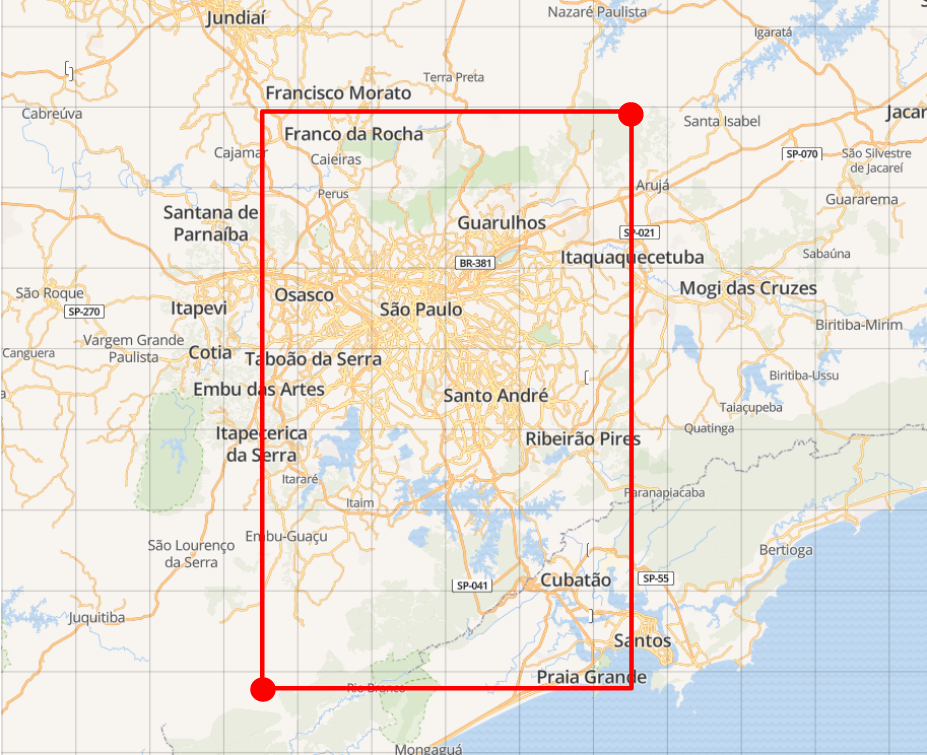
\includegraphics[width=1\linewidth]{figures/sp_bb.png}
		\caption{São Paulo}
		\label{fig:saopaulo_bounding_box}
	\end{subfigure}%
	\quad
	\begin{subfigure}[t]{0.3\textwidth}
		\centering
		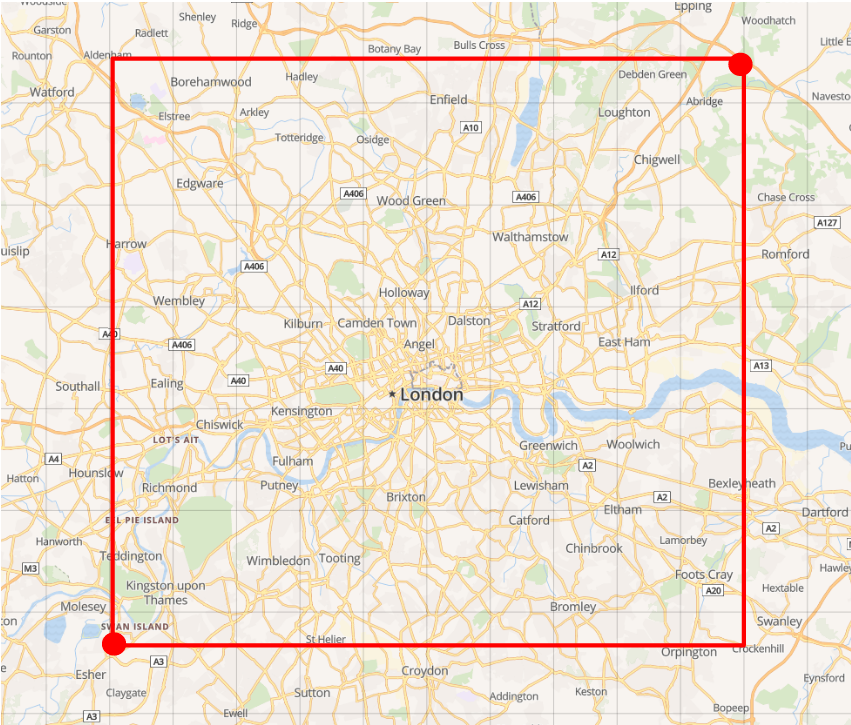
\includegraphics[width=1\linewidth]{figures/london_bb.png}
		\caption{London}
		\label{fig:london_bounding_box}
	\end{subfigure}
	\quad
	\begin{subfigure}[t]{0.3\textwidth}
		\centering
		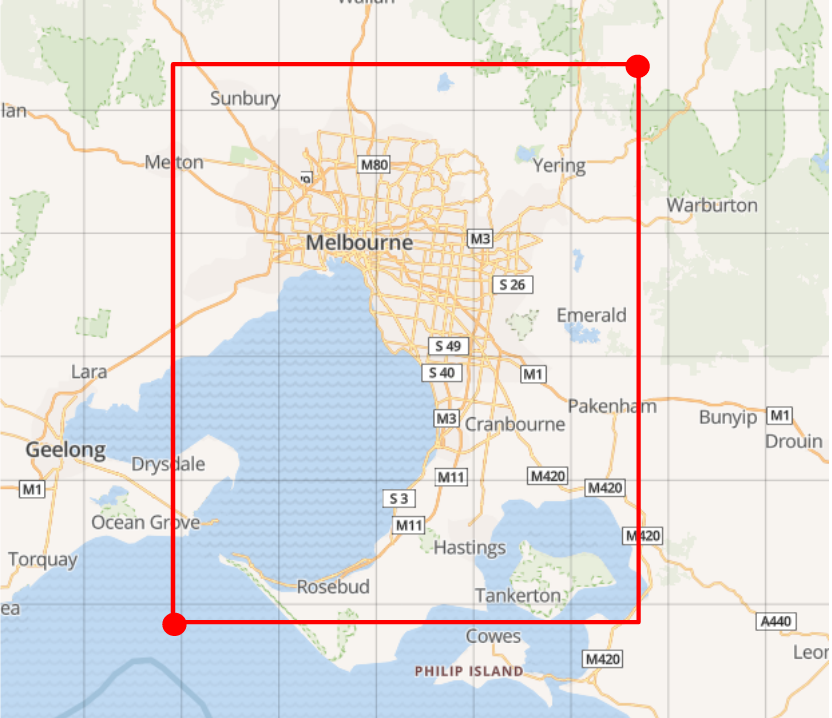
\includegraphics[width=1\linewidth]{figures/melbourne_bb.png}
		\caption{Melbourne}
		\label{fig:melbourne_bounding_box}
	\end{subfigure}
	
	\medskip
	
	\begin{subfigure}[t]{0.42\textwidth}
		\centering
		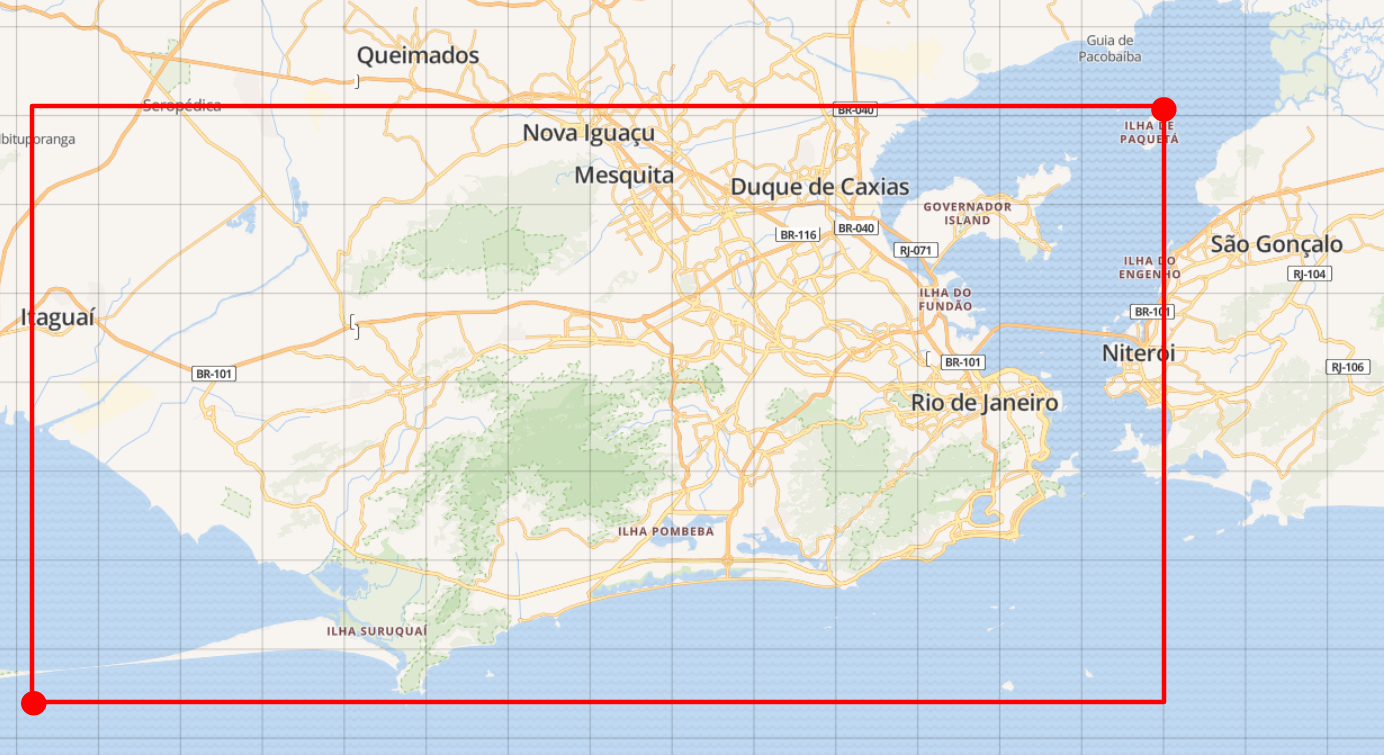
\includegraphics[width=1\linewidth]{figures/rio_bb.png}
		\caption{Rio de Janeiro}
		\label{fig:riodejaneiro_bounding_box}
	\end{subfigure}
	\quad
	\begin{subfigure}[t]{0.38\textwidth}
		\centering
		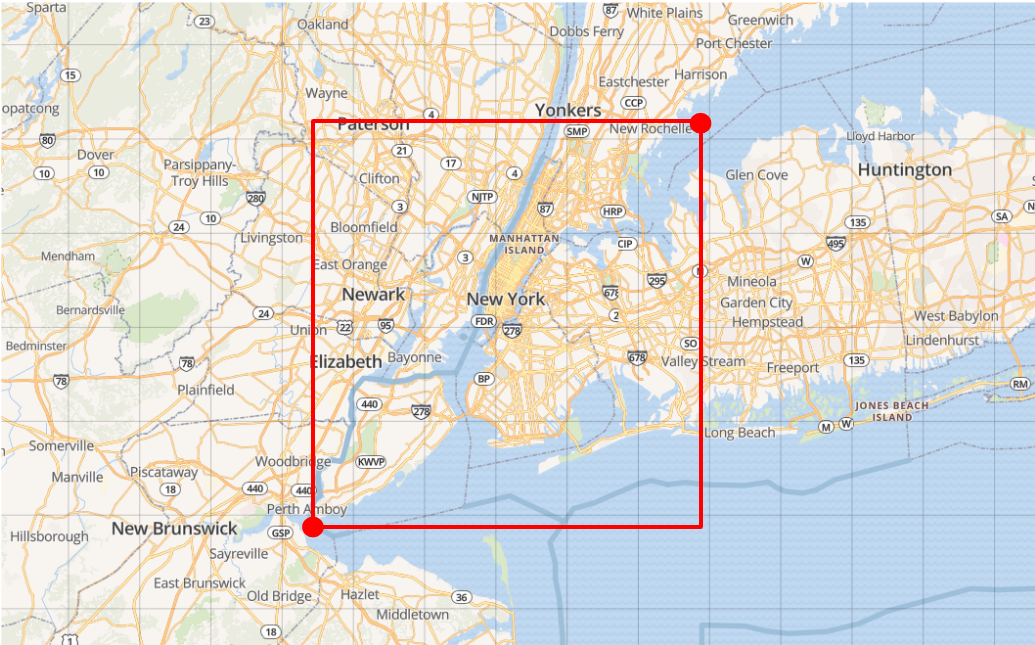
\includegraphics[width=1\linewidth]{figures/newyork_bb.png}
		\caption{New York}
		\label{fig:newyork_bounding_box}
	\end{subfigure}
	\caption{Search Bounding-boxes for the data collection}
	\label{fig:bounding_boxes}
\end{figure}

\begin{table}[b]
	\centering
	\setlength\extrarowheight{3pt}
	\caption{Collecting Bounding-boxes Coordinates (South-West and North-East)}
	\label{tab:bbs_points}
	\begin{tabular}{l|c|c}
		\hline
		\multicolumn{1}{c|}{\textbf{City}} & \textbf{South-West} & \textbf{North-East} \\ \hline
		\textbf{Rio de Janeiro} & (-43.7950599, -23.0822288) & (-43.0969042, -22.7460327) \\
		\textbf{São Paulo} & (-46.825514, -24.0082209) & (-46.3650844, -23.3566039) \\
		\textbf{New York City} & (-74.2590899, 40.4773991) & (-73.7002721, 40.9175771) \\
		\textbf{London} & (-0.3514683, 51.3849401) & (0.148271, 51.6723432) \\
		\textbf{Melbourne} & (144.5937418, -38.4338593) & (145.5125288, -37.5112737) \\ \hline
	\end{tabular}
\end{table}

Taking a careful observation into to coordinates used to each bounding-box, we can affirm that Rio de Janeiro present the broadest bounding-box comparatively to the others cities.

In the first attempts to study the geographic distribution in our datasets, we discover that not all tweets had a precise coordinate attached to it. Nonetheless, there were cases where tweets from other cities were collected to our datasets and this phenomenon is not supposed to happen when the collection method is based in geo-located characteristics. By studying the Twitter mobile application, we found out that a user can tag himself in the tweet by two different ways: (1) a user can activate the GPS in the mobile application and associate to the tweet his precisely geo-location; (2) a user can choose a place from a predefined list provide by Twitter and associate the place to the tweet.

The second method of tagging the geo-location to the tweet can arise some conflicts when this kind of tweets is used to perform scientific studies or even development of system to help the cities in the regularization, control and improvement of its services. Having this in consideration, it was necessary to understand how the Twitter Streaming API works and what kind of heuristics follows in order to retrieve this type of tweets. Hence, the documentation~\footnote{\url{https://dev.twitter.com/streaming/overview/request-parameters\#locations} (last visited on 17 June, 2017)} enhances two different heuristics:

\begin{enumerate}
	\item If the coordinates field is populated, the values there will be tested against the bounding-box;
	\item If the coordinates field is empty but place is populated, the region defined in place is checked for intersections against the locations bounding-box. Any overlapping areas will yield a positive match.
\end{enumerate}

The first heuristic only happens if a user is able/willing to tag a post with his precise geo-location associated with it; otherwise, the user can tag the post associated with a place and in this case the second heuristic is applied. 
Each place contained in the previous mentioned list, which is provided by Twitter, is composed by a bounding-box, and if any piece of it overlaps the bounding-box used in the collecting process, then a positive match is yielded and the tweet is retrieved. For example, if a tweet has a place such as Brazil and our filter bounding-box is defined for Rio de Janeiro, all tweets from place Brazil will be in our dataset, regardless the fact some tweets are posted elsewhere, such as in the city of Manaus, very far away from Rio de Janeiro.

This restriction required the development of a external layer which was responsible for the filter of tweets located outside the area of each city. To built this so, it was necessary \textit{a posteriori} information and, thus, we extract the Twitter default bounding-box of each city appealing to the tweets \textit{place} field. Such information was then used as the limit area in order to filter out tweets which \textit{coordinates} field was not populated. These bounding-boxes, the Twitter default ones, are listed in Table~\ref{tab:bbs_filter} and its corresponding visualization is the biggest rectangle demonstrated in Figures~\ref{fig:rio_sp_geographical_distribution} (subfigures~\ref{subfig:riodejaneiro_bounding_boxes} and~\ref{subfig:saopaulo_bounding_boxes}) and~\ref{fig:nyc_london_melbourne_geographical_distribution} (subfigures~\ref{subfig:nyc_bounding_boxes},~\ref{subfig:london_bounding_boxes} and~\ref{subfig:melbourne_bounding_boxes}).

\begin{table}[htbp]
	\centering
	\setlength\extrarowheight{3pt}
	\caption{Twitter Default Bounding-boxes Coordinates (South-West and North-East)}
	\label{tab:bbs_filter}
	\begin{tabular}{l|c|c}
		\hline
		\multicolumn{1}{c|}{\textbf{City}} & \textbf{South-West} & \textbf{North-East} \\ \hline
		\textbf{Rio de Janeiro} & (-43.795449, -23.08302) & (-43.087707, -22.739823) \\
		\textbf{São Paulo} & (-46.826039, -24.008814) & (-46.365052, -23.356792) \\
		\textbf{New York City} & (-74.255641, 40.495865) & (-73.699793, 40.91533) \\
		\textbf{London} & (-0.510365, 51.286702) & (0.334043, 51.691824) \\
		\textbf{Melbourne} & (144.593742, -38.433859) & (145.512529, -37.511274) \\ \hline
	\end{tabular}
\end{table}

The final volume of tweets located inside and outside the cities correspondent bounding-boxes are presented in Table~\ref{tab:geographic_counts_bb}. Alongside with the location analysis, the language count was also performed since future experiments only took into consideration tweets with the native language of the city in study and not foreign ones. In the abovementioned table (\ref{tab:geographic_counts_bb}) it is possible to verify a vast difference regarding the activity on Twitter in Rio de Janeiro. Numbers tell that such activity, with respect to geo-located tweets, is almost two times more than São Paulo, four times London and twenty five times Melbourne. A possible justification for this noticeable difference may be associated to the area of the bounding-box used in the collection process, but, on the other hand, according to some sources related to the demographic measures, for the case Rio De Janeiro \textit{versus} São Paulo, the population volume has an opposite behavior, where São Paulo~\footnote{\url{https://cidades.ibge.gov.br/v4/brasil/sp/sao-paulo/panorama} (last visited on 17 June, 2017)} has almost 12 millions habitants while Rio de Janeiro~\footnote{\url{https://cidades.ibge.gov.br/v4/brasil/rj/rio-de-janeiro/panorama} (last visited on 17 June, 2017)} has 6 million. Having only this amount of information it is impossible, at the moment, formulate a explanation to this phenomenon.

\begin{table}[htbp]
	\centering
	\caption[Datasets composition according bounding-box analysis]{Datasets composition after verification of the tweets inside the corresponding bounding-box}
	\label{tab:geographic_counts_bb}
	\resizebox{\textwidth}{!}{\begin{tabular}{l|c|cl|cl|cl|cl|cl}
			\hline
			\multicolumn{1}{c|}{\multirow{2}{*}{\textbf{City}}} & \multirow{2}{*}{\textbf{All}} & \multicolumn{2}{c|}{\textbf{PT/EN}} & \multicolumn{2}{c|}{\textbf{Non-PT/EN}} & \multicolumn{2}{c|}{\textbf{\begin{tabular}[c]{@{}c@{}}In\\ Bounding-Box\end{tabular}}} & \multicolumn{2}{c|}{\textbf{\begin{tabular}[c]{@{}c@{}}Out\\ Bounding-Box\end{tabular}}} & \multicolumn{2}{c|}{\textbf{\begin{tabular}[c]{@{}c@{}}PT/EN and In\\ Bounding-Box\end{tabular}}} \\ \cline{3-12} 
			\multicolumn{1}{c|}{} &  & \textbf{No. tweets} & \multicolumn{1}{c|}{\textbf{\%}} & \textbf{No. tweets} & \multicolumn{1}{c|}{\textbf{\%}} & \textbf{No. tweets} & \multicolumn{1}{c|}{\textbf{\%}} & \textbf{No. tweets} & \multicolumn{1}{c|}{\textbf{\%}} & \textbf{No. tweets} & \multicolumn{1}{c}{\textbf{\%}} \\ \hline
			\textbf{Rio de Janeiro} & 18,803,774 & 15,906,680 & 84,59\% & 2,897,094 & 15,41\% & 12,976,048 & 69,01\% & 5,827,726 & 30,99\% & 11,060,136 & 58,82\% \\
			\textbf{São Paulo} & 9,319,624 & 7,203,115 & 77,29\% & 2,116,509 & 22,71\% & 6,237,427 & 66,93\% & 3,082,197 & 33,07\% & 4,886,626 & 52,43\% \\
			\textbf{New York City} & 8,507,145 & 7,260,829 & 85,35\% & 1,246,316 & 14,65\% & 6,972,312 & 81,96\% & 1,534,833 & 18,04\% & 5,956,355 & 70,02\% \\
			\textbf{London} & 5,596,551 & 4,774,310 & 85,31\% & 822,241 & 14,69\% & 4,752,918 & 84,93\% & 843,633 & 15,07\% & 4,040,092 & 72,19\% \\
			\textbf{Melbourne} & 789,927 & 669,435 & 84,75\% & 120,492 & 15,25\% & 742,946 & 94,05\% & 46,981 & 5,95\% & 629,424 & 79,68\% \\ \hline
		\end{tabular}}
	\end{table}

Later, after the filtering process, we tried to understand the volume, as well as the location of each tweet. Through this kind of analysis it was possible to find out that a tweet which \textit{coordinates }field was empty and is, actually, represented with a bounding-box, can also be a specific place, i.e. a place that has a precise coordinate. Not all places were represented by a bounding-box in which each point that composed it are different. An example to that is \texttt{Estádio do Maracanã} which although being represented by a bounding-box, all four points are equal. A division was made considering this three types of location - (1) bounding-box with four different points; (2) bounding-box with four equal points; (3) precise coordinate - in order to have a perception of how different specific places and bounding-boxes as so which is the volume of tweets that are related to it.

\begin{table}[htbp]
	\centering
	\caption{Volume of tweets for each type of geo-location}
	\label{tab:volume_geolocation}
	\resizebox{\textwidth}{!}{\begin{tabular}{l|c|ccc|ccc|ccc}
			\hline
			\multicolumn{1}{c|}{\multirow{2}{*}{\textbf{City}}} & \multirow{2}{*}{\textbf{Total}} & \multicolumn{3}{c|}{\textbf{Bounding-boxes}} & \multicolumn{3}{c|}{\textbf{Specific Places}} & \multicolumn{3}{c|}{\textbf{Precisely}} \\ \cline{3-11} 
			\multicolumn{1}{c|}{} &  & \multicolumn{1}{c|}{\textbf{Distinct}} & \multicolumn{1}{c|}{\textbf{No. Tweets}} & \textbf{Percentage (\%)} & \multicolumn{1}{c|}{\textbf{Distinct}} & \multicolumn{1}{c|}{\textbf{No. Tweets}} & \textbf{Percentage (\%)} & \multicolumn{1}{c|}{\textbf{Distinct}} & \multicolumn{1}{c|}{\textbf{No. Tweets}} & \textbf{Percentage (\%)} \\ \hline
			\textbf{Rio de Janeiro} & 11060136 & 297 & 10237280 & 92,56\% & 11159 & 49440 & 0,45\% & 163748 & 773416 & 6,99\% \\
			\textbf{São Paulo} & 4886626 & 325 & 4284795 & 87,68\% & 7189 & 21022 & 0,43\% & 100028 & 580809 & 11,89\% \\
			\textbf{New York City} & 5956355 & 328 & 4210854 & 70,70\% & 16078 & 85204 & 1,43\% & 138123 & 1660297 & 27,87\% \\
			\textbf{London} & 4040092 & 53 & 3196043 & 79,11\% & 8123 & 53412 & 1,32\% & 95317 & 790637 & 19,57\% \\
			\textbf{Melbourne} & 629424 & 22 & 523870 & 83,23\% & 0 & 0 & 0,00\% & 21826 & 105554 & 16,77\% \\ \hline
		\end{tabular}}
	\end{table}
	
The final counts of the analysis for each identified type of geo-location are presented in Table~\ref{tab:volume_geolocation}. Looking at the numbers it is possible to conclude some facts applicable to all cities. Citizens tend to geo-locate themselves with a location which has variable bounding-box size since more than 70\% of the tweets are of this type. Furthermore, only a few percentage of tweets, between 0\% and 1.43\%, are located in specific places, although the existence of a higher number of distinct specific places comparatively to the bounding-boxes with variable size, with exception of Melbourne that has zero specific places in our dataset. Other interesting point to enhance is the considerable percentage of tweets with precise location (i.e. tweets that people tagged himself using the GPS). The Brazilian cities proved to be less supportive of precisely located tweets, while the English cities were more contributive. The distribution of each type of geo-located tweet is illustrated in Figures~\ref{fig:rio_sp_geographical_distribution} and~\ref{fig:nyc_london_melbourne_geographical_distribution}. The variable bounding-boxes are showed in ~\ref{subfig:saopaulo_bounding_boxes},~\ref{subfig:riodejaneiro_bounding_boxes},~\ref{subfig:nyc_bounding_boxes},~\ref{subfig:london_bounding_boxes} and~\ref{subfig:melbourne_bounding_boxes} proving that our filter method was able to correctly agglomerate places that were, indeed, inside of the Twitter default bounding-boxes. In~\ref{subfig:saopaulo_markers},~\ref{subfig:riodejaneiro_markers},~\ref{subfig:nyc_markers},~\ref{subfig:london_markers} and~\ref{subfig:melbourne_markers} is illustrated the distribution of the specific places found out in our datasets for each city. A particular point identified was the absence of specific places in Melbourne and the limited places in a certain area of London. With a first look at the image of London, there may be doubts about the results concerning the filter method, however the bounding-box used to that process was the same in both cases, and so the only viable explanation for such result is the absence of specific locations for that area in the predefined list of places provided by the Twitter applications. Lastly, in~\ref{subfig:saopaulo_points},~\ref{subfig:riodejaneiro_points},~\ref{subfig:nyc_points},~\ref{subfig:london_points} and~\ref{subfig:melbourne_points} is illustrated the distribution of precisely located tweets. Through a careful observation in this distribution it was possible the arising of another doubt relatively to the first aforementioned heuristic of the Twitter Streaming API. There were tweets retrieved that not matched the bounding-box used in the collection process and this fact conducts to uncertainty and mistrust regarding the performance of this type of collection available on Twitter. 

\begin{figure}[htbp]
	\centering
	\begin{subfigure}[htbp]{0.4\textwidth}
		\centering
		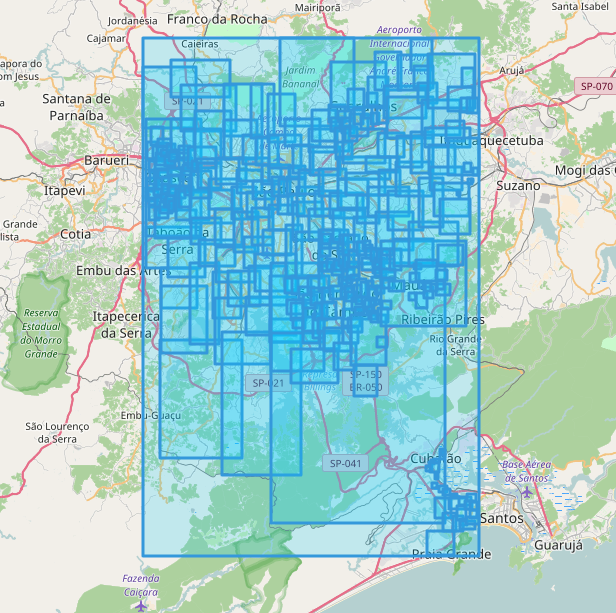
\includegraphics[width=1\linewidth]{figures/sp_bbs.png}
		\caption{}
		\label{subfig:saopaulo_bounding_boxes}
	\end{subfigure}
	\quad
	\begin{subfigure}[htbp]{0.5\textwidth}
		\centering
		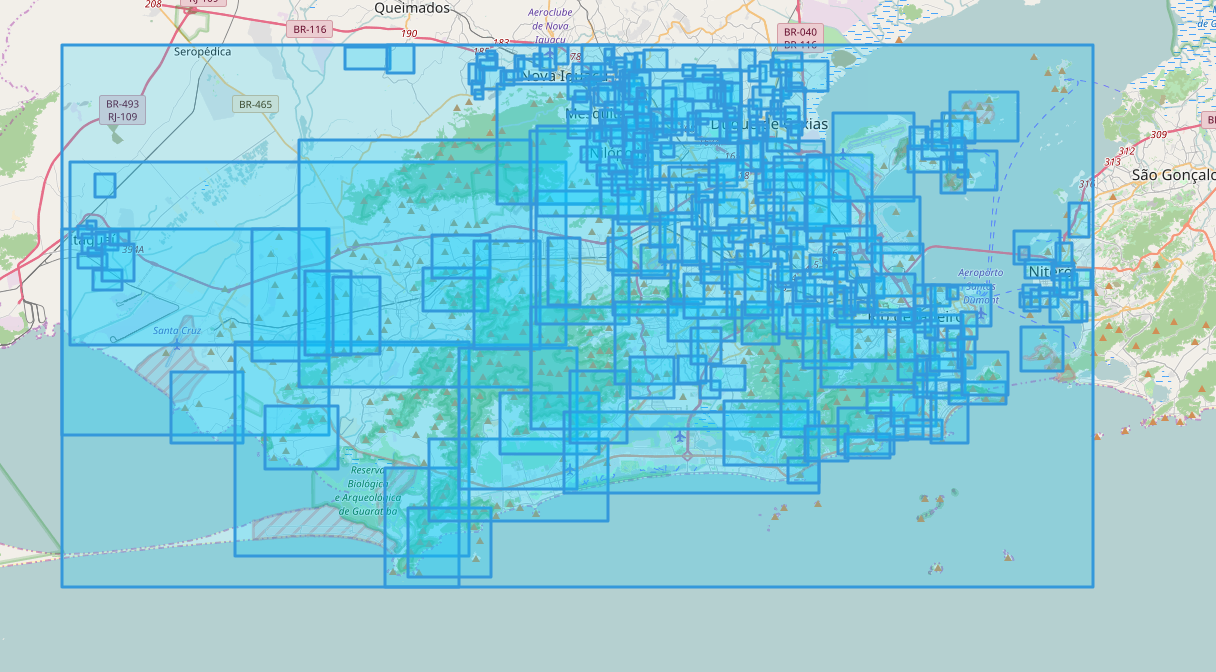
\includegraphics[width=1\linewidth]{figures/rio_bbs.png}
		\caption{}
		\label{subfig:riodejaneiro_bounding_boxes}
	\end{subfigure}
	
	\medskip
	
	\begin{subfigure}[htbp]{0.4\textwidth}
		\centering
		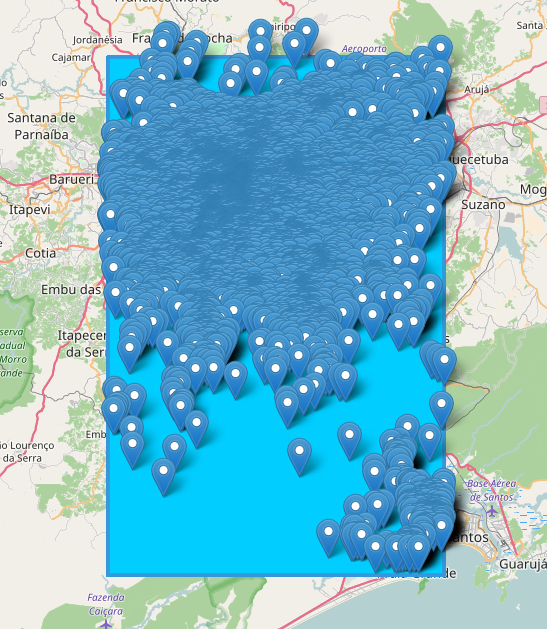
\includegraphics[width=1\linewidth]{figures/sp_markers.png}
		\caption{}
		\label{subfig:saopaulo_markers}
	\end{subfigure}
	\quad
		\begin{subfigure}[htbp]{0.5\textwidth}
			\centering
			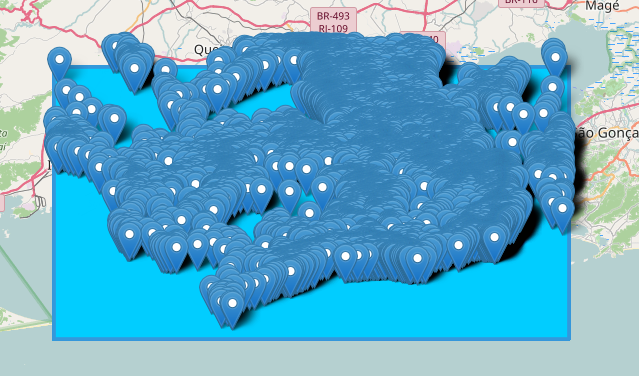
\includegraphics[width=1\linewidth]{figures/rio_markers.png}
			\caption{}
			\label{subfig:riodejaneiro_markers}
		\end{subfigure}
		
	\medskip
	
	\begin{subfigure}[htbp]{0.4\textwidth}
		\centering
		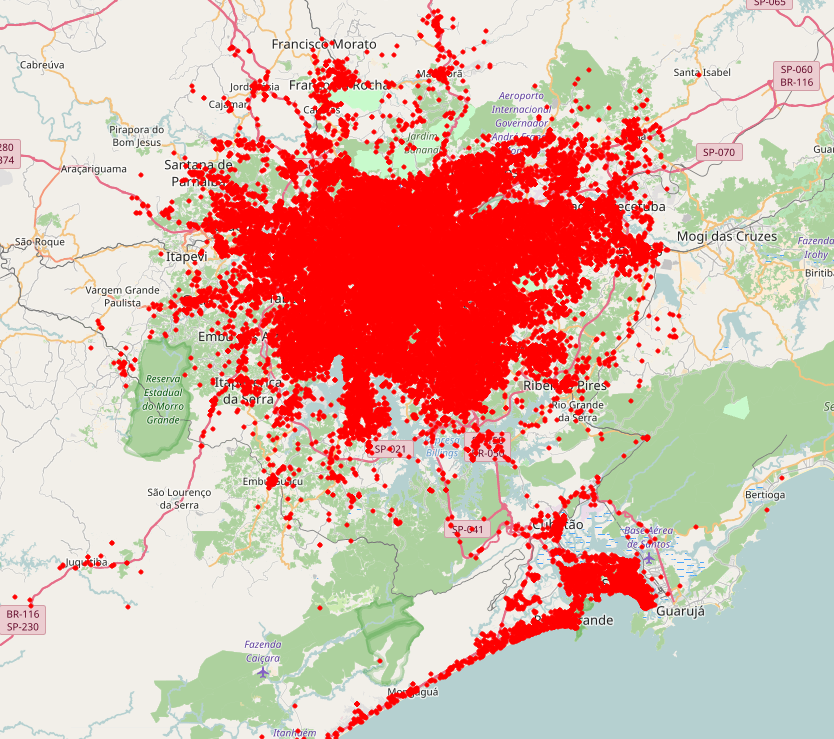
\includegraphics[width=1\linewidth]{figures/sp_points.png}
		\caption{}
		\label{subfig:saopaulo_points}
	\end{subfigure}
	\quad
	\begin{subfigure}[htbp]{0.5\textwidth}
		\centering
		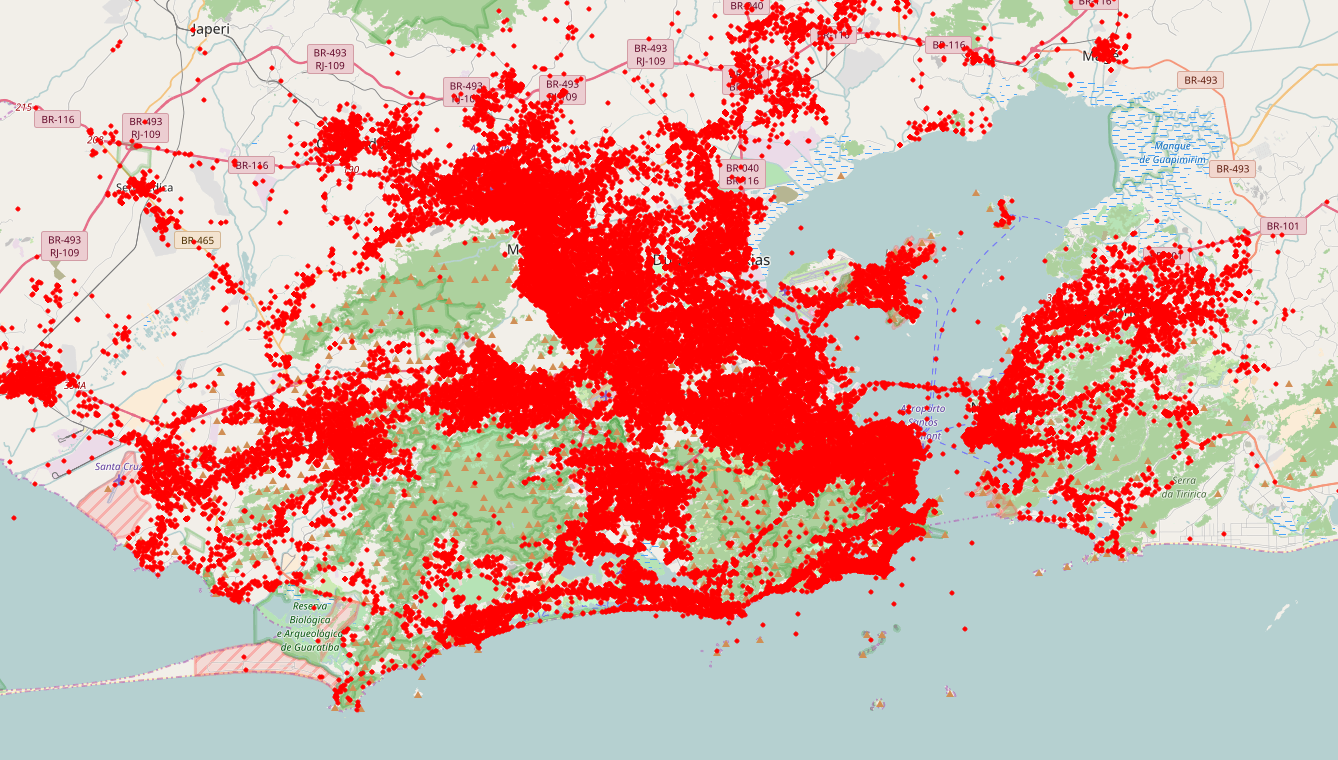
\includegraphics[width=1\linewidth]{figures/rio_points.png}
		\caption{}
		\label{subfig:riodejaneiro_points}
	\end{subfigure}
	
	\caption[Exploratory analysis in Brazilian cities]{São Paulo (a, c, e) and Rio de Janeiro (b, d, f) Geographical Distributions: (a, b) Bounding-boxes of places (c, d) Specific places (e, f) Geo-tagged tweets}
	\label{fig:rio_sp_geographical_distribution}
\end{figure}

\begin{figure}[htbp]
	\centering
	\begin{subfigure}[htbp]{0.3\textwidth}
		\centering
		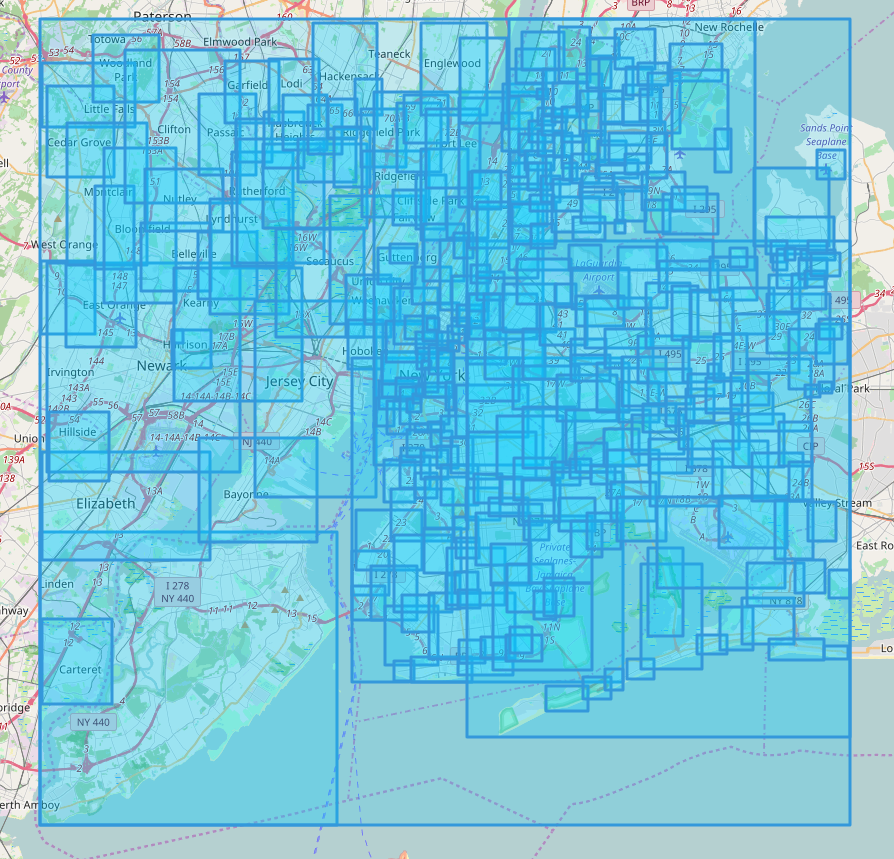
\includegraphics[width=1\linewidth]{figures/nyc_bbs.png}
		\caption{}
		\label{subfig:nyc_bounding_boxes}
	\end{subfigure}
	\quad
	\begin{subfigure}[htbp]{0.3\textwidth}
		\centering
		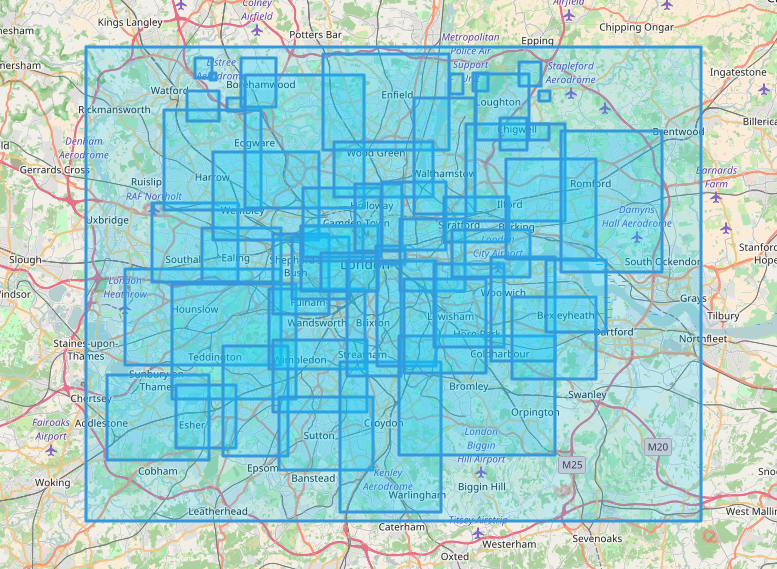
\includegraphics[width=1\linewidth]{figures/london_bbs.png}
		\caption{}
		\label{subfig:london_bounding_boxes}
	\end{subfigure}
	\quad
	\begin{subfigure}[htbp]{0.3\textwidth}
		\centering
		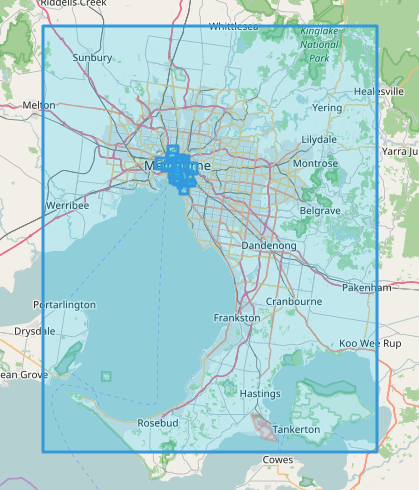
\includegraphics[width=1\linewidth]{figures/melbourne_bbs.png}
		\caption{}
		\label{subfig:melbourne_bounding_boxes}
	\end{subfigure}
			
	\medskip
	
	\centering
	\begin{subfigure}[htbp]{0.3\textwidth}
		\centering
		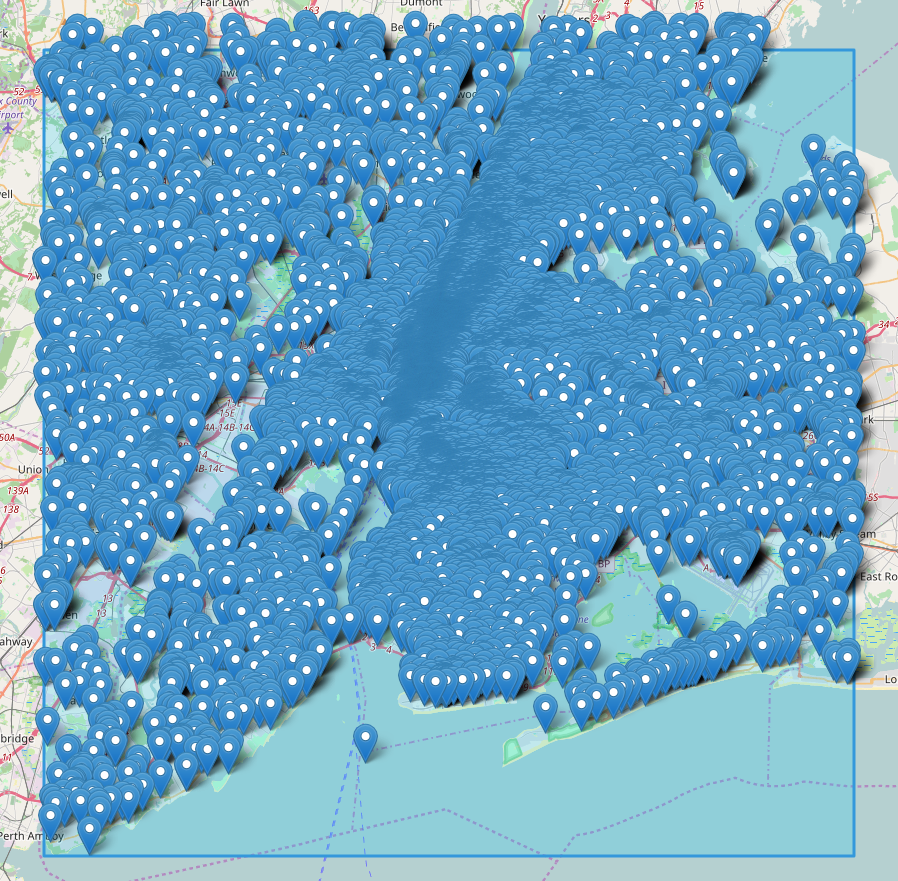
\includegraphics[width=1\linewidth]{figures/nyc_markers.png}
		\caption{}
		\label{subfig:nyc_markers}
	\end{subfigure}
	\quad
	\begin{subfigure}[htbp]{0.3\textwidth}
		\centering
		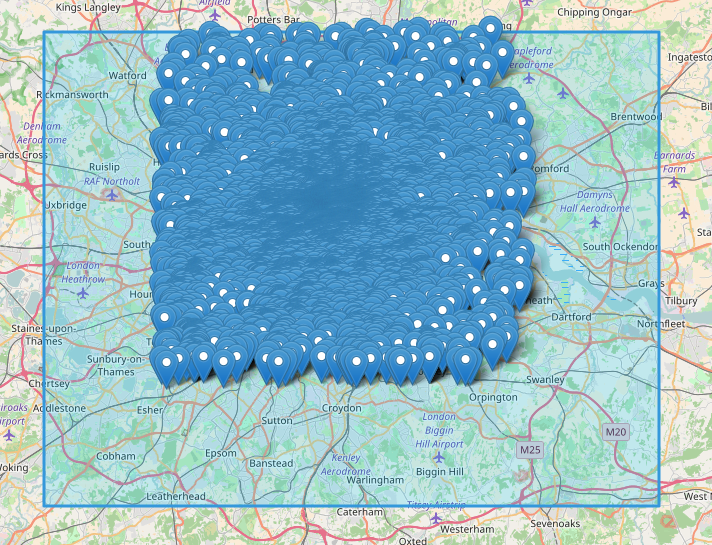
\includegraphics[width=1\linewidth]{figures/london_markers.png}
		\caption{}
		\label{subfig:london_markers}
	\end{subfigure}
	\quad
	\begin{subfigure}[htbp]{0.3\textwidth}
		\centering
		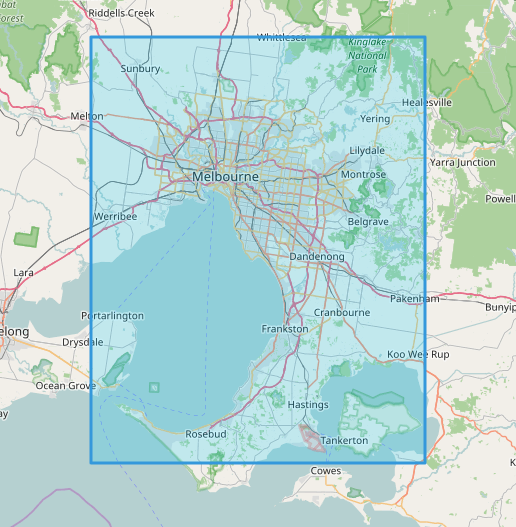
\includegraphics[width=1\linewidth]{figures/melbourne_markers.png}
		\caption{}
		\label{subfig:melbourne_markers}
	\end{subfigure}
	
	\medskip
	\centering
	\begin{subfigure}[htbp]{0.3\textwidth}
		\centering
		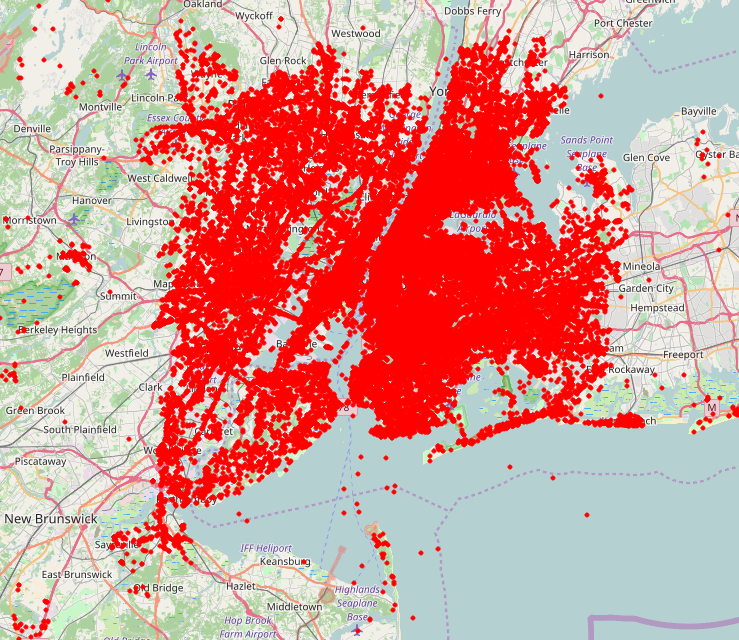
\includegraphics[width=1\linewidth]{figures/nyc_points.png}
		\caption{}
		\label{subfig:nyc_points}
	\end{subfigure}
	\quad
	\begin{subfigure}[htbp]{0.3\textwidth}
		\centering
		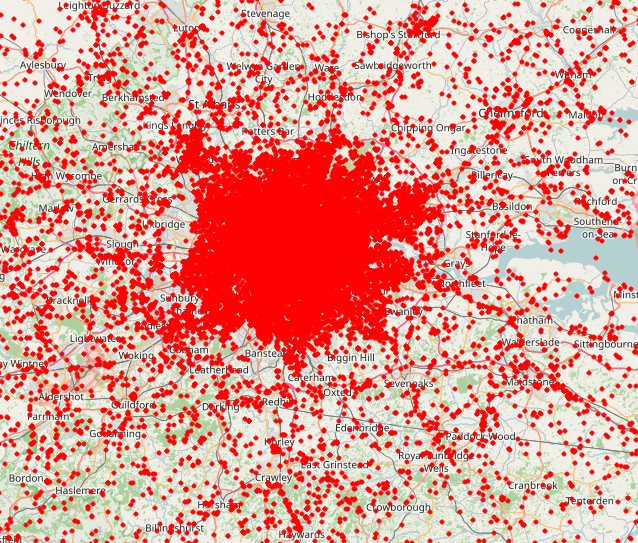
\includegraphics[width=1\linewidth]{figures/london_points.png}
		\caption{}
		\label{subfig:london_points}
	\end{subfigure}
	\quad
	\begin{subfigure}[htbp]{0.3\textwidth}
		\centering
		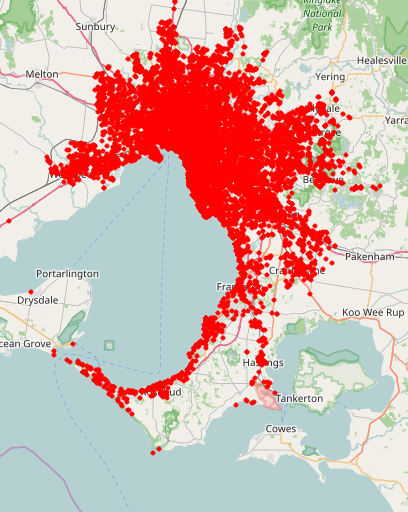
\includegraphics[width=1\linewidth]{figures/melbourne_points.png}
		\caption{}
		\label{subfig:melbourne_points}
	\end{subfigure}
	
	\caption[Exploratory analysis in English-speaking cities]{New York City (a, d, g), London (b, e, h) Geographical Distributions: (a, b) Bounding-boxes of places (c, d) Specific places (e, f) Geo-tagged tweets}
	\label{fig:nyc_london_melbourne_geographical_distribution}
\end{figure}

\section{Temporal Frequencies}

Another interesting analysis in our datasets concerns the temporal distribution of the data. The volume of tweets posted per hour, per day, as well as the activity by day-of-the-week or hour-of-the-day are statistics that enable the possibility of finding out patterns or variations which can be correlated to some events or incidents happening in a city.

\begin{figure}[htbp]
	\centering
	\begin{subfigure}[htbp]{0.8\textwidth}
		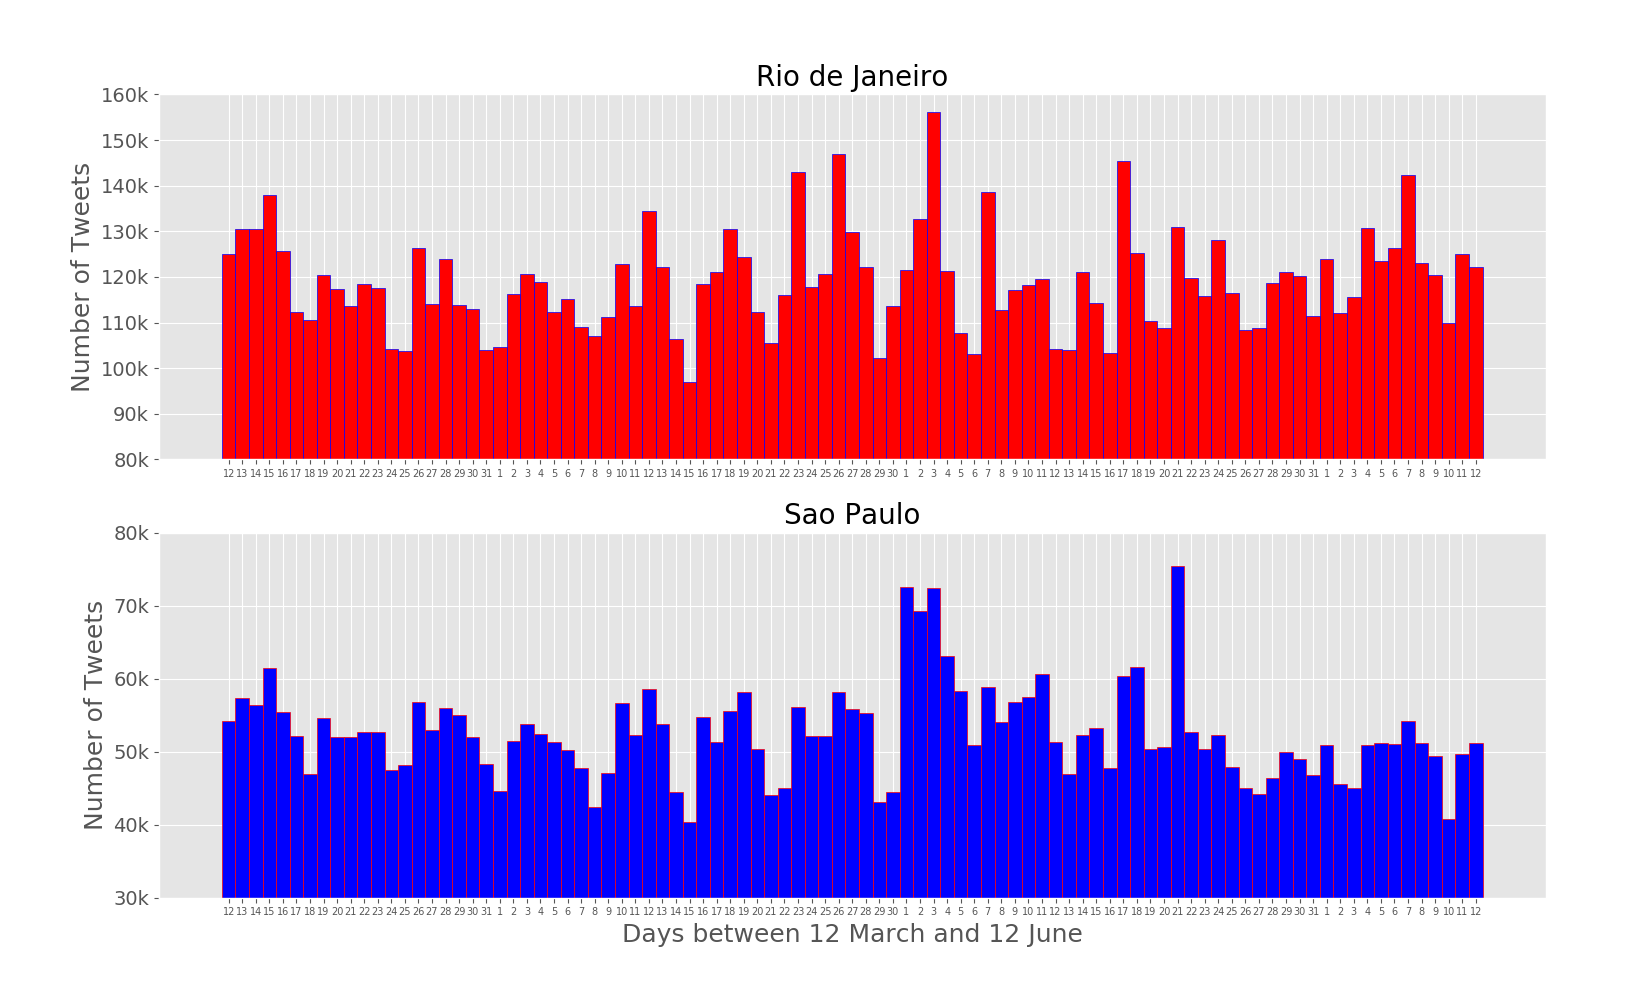
\includegraphics[width=\linewidth]{figures/rio_sp_whole_months.png}
		\caption{}
		\label{subfig:portuguese_cities_whole_months} 
	\end{subfigure}
	
	\begin{subfigure}[htbp]{0.8\textwidth}
		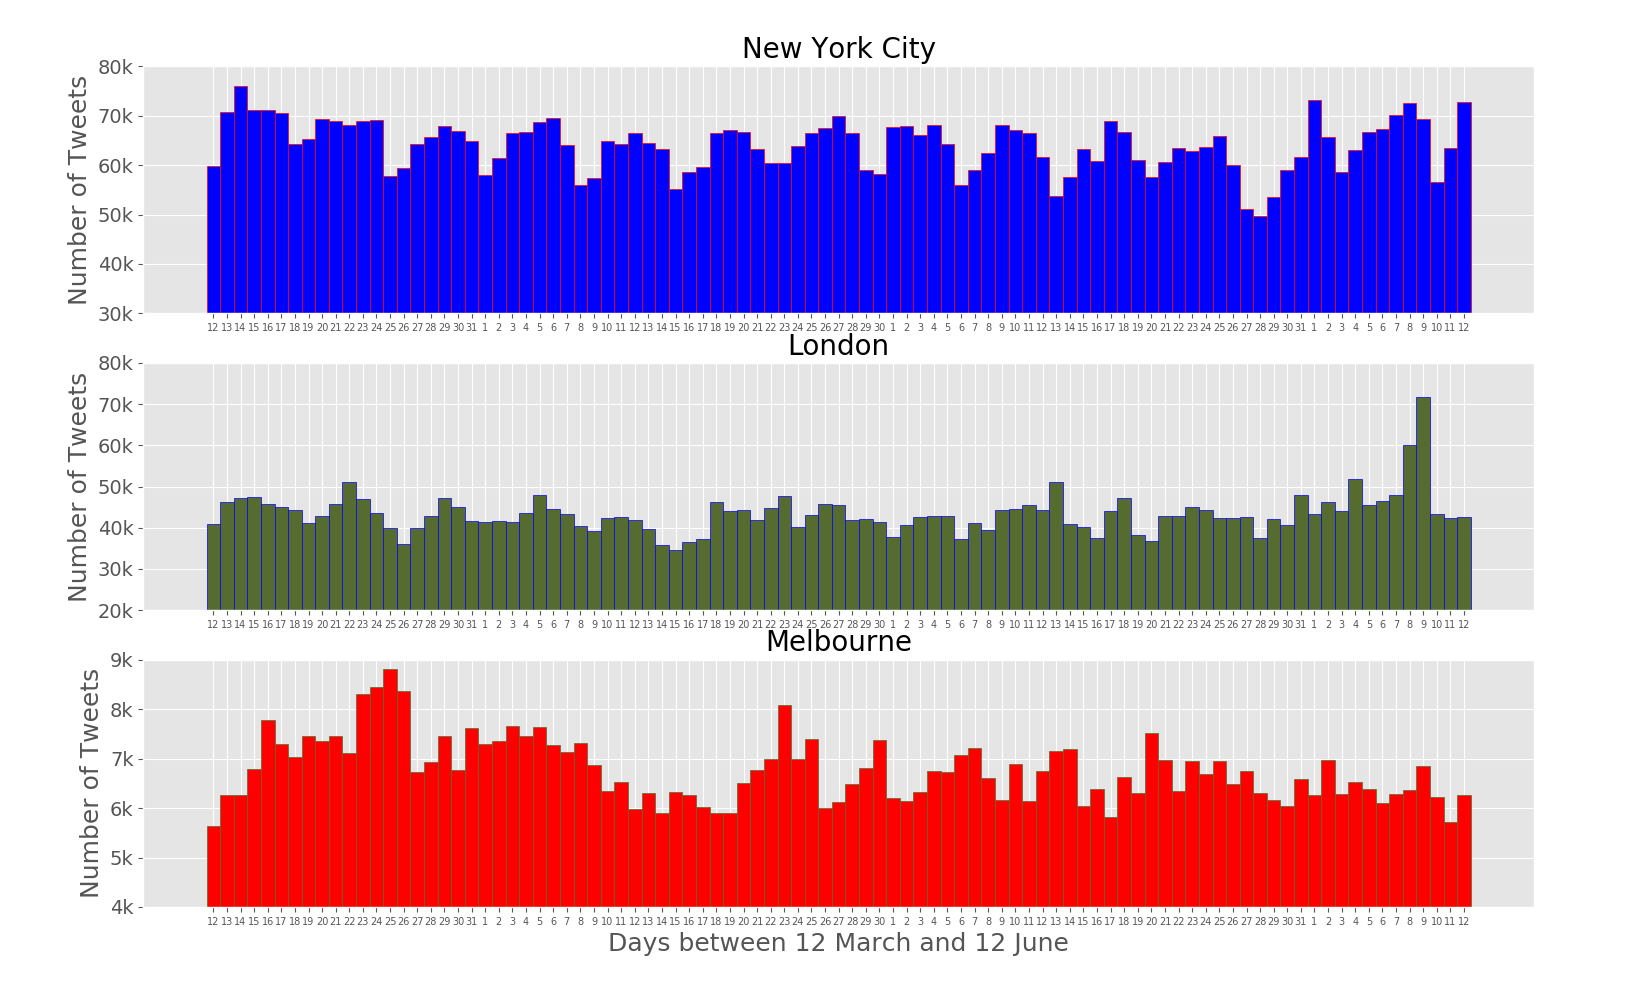
\includegraphics[width=\linewidth]{figures/nyc_london_melbourne_whole_months.png}
		\caption{}
		\label{subfig:english_cities_whole_months}
	\end{subfigure}
	
	\caption[Daily volume of tweets]{Daily volume of tweets (a) Rio de Janeiro and São Paulo - Portuguese Cities (b) New York City, London and Melbourne - English Cities}
	\label{fig:daily_distribution}
\end{figure}

During and after remarkable events, citizens are impelled to share their feelings, opinions or even report their safety and well-being conditions (e.g. in cases of terrorist attack) through mobile applications. This share of information increases the activity of social media platforms, which can be potentially used for the identification of uncommon events. Figure~\ref{fig:daily_distribution} illustrates the daily distribution of all cities for the period of collection, three whole months, between 12 March and 12 June, 2017. The Brazilian cities present high level of variation between consecutive days (with the volume varying in a tens of thousands of tweets) and so the task of identifying remarkable events turns out to be much harder. On the other hand, the English speaking cities in our study are very similar, with exception of Melbourne whose activity is very low comparatively to the other cities (New York City and London). In the particular case of London, we can identify an abrupt increase of volume during days 8 and 9 of June. With the support of external sources such as news websites, we learnt about the United Kingdom General Elections 2017~\footnote{\url{https://www.theguardian.com/politics/general-election-2017} (Accessed on 17/06/2017)} occurred on that period which suggests that an increase of the Twitter activity might be associated with that event. 

\begin{figure}[htbp]
    \centering
    \begin{subfigure}[htbp]{0.45\textwidth}
        \centering
        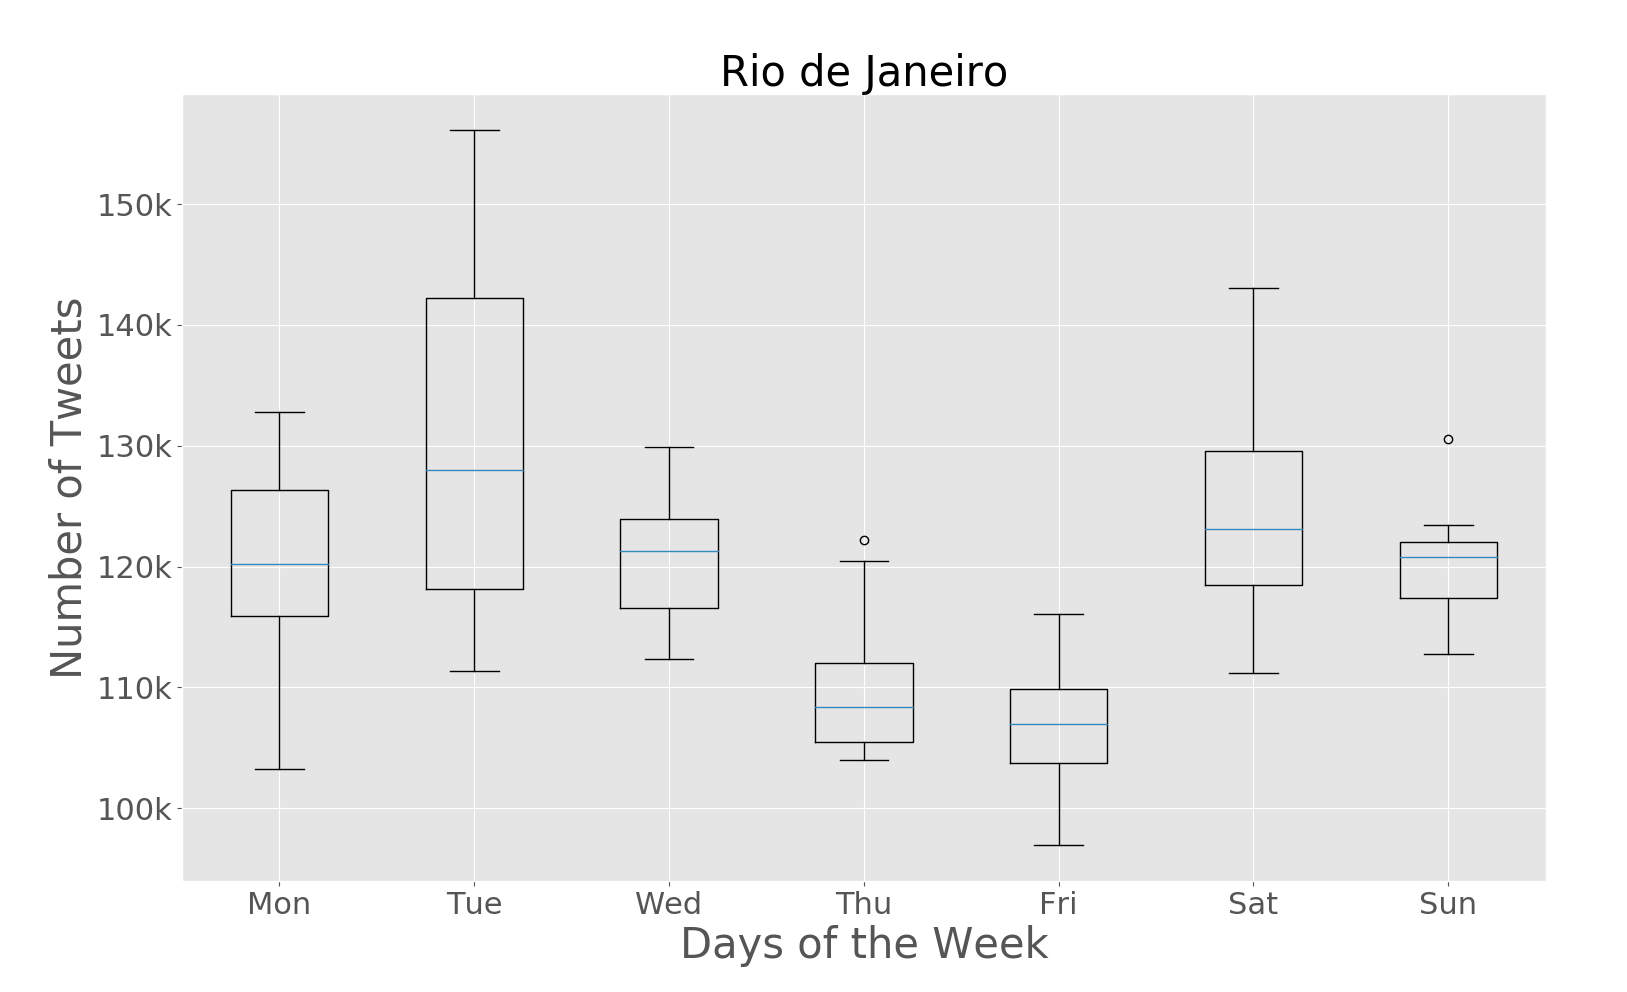
\includegraphics[width=1\linewidth]{figures/rio_box_plt_day_of_week.png}
        \caption{}
        \label{subfig:riodejaneiro_box_plot_day_of_week}
    \end{subfigure}%
    \quad
    \begin{subfigure}[htbp]{0.45\textwidth}
        \centering
        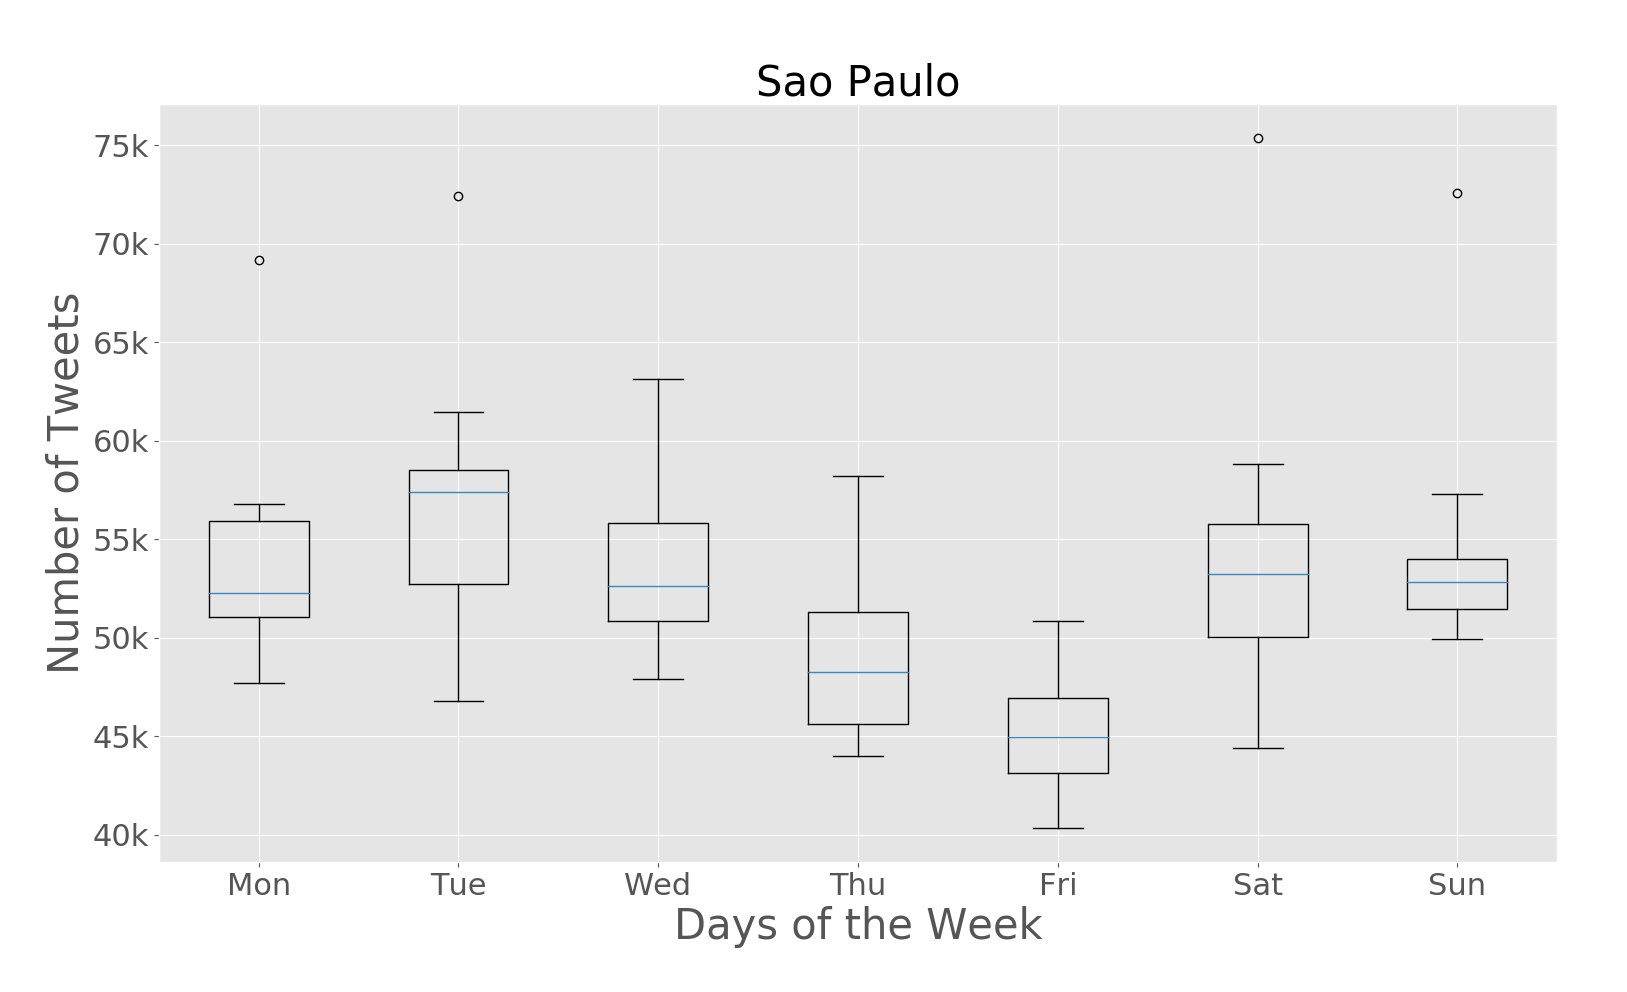
\includegraphics[width=1\linewidth]{figures/sp_box_plt_day_of_week.png}
        \caption{}
        \label{subfig:saopaulo_box_plot_day_of_week}
    \end{subfigure}

    \medskip

    \begin{subfigure}[htbp]{0.45\textwidth}
        \centering
        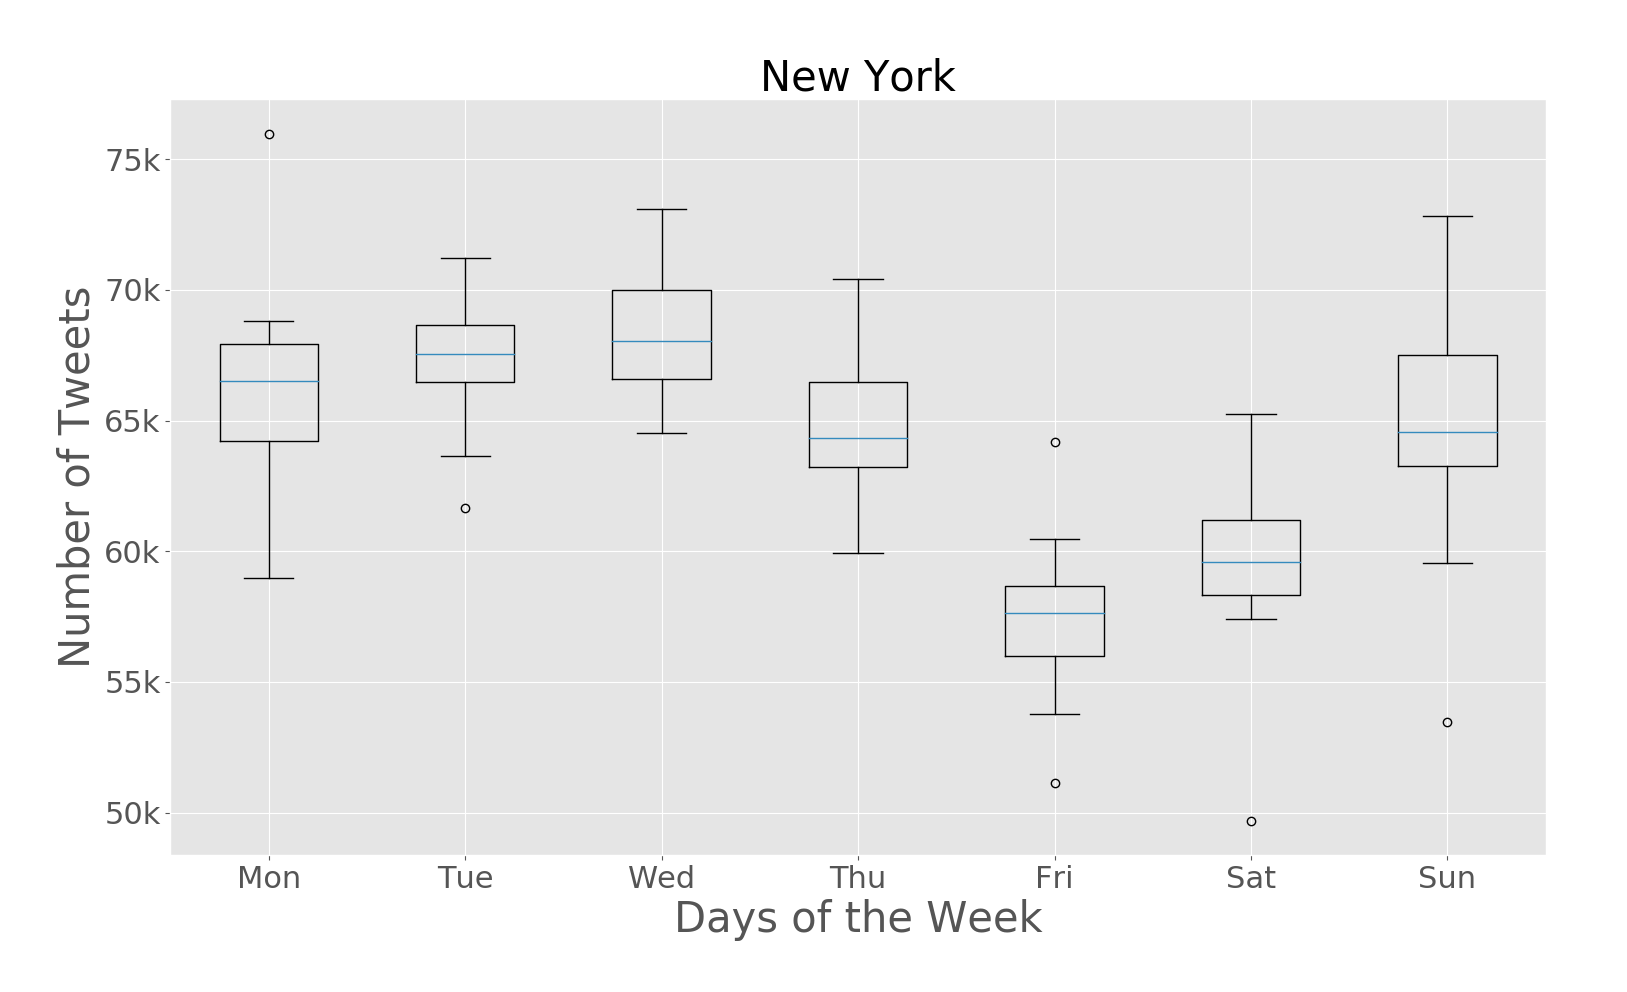
\includegraphics[width=1\linewidth]{figures/nyc_box_plt_day_of_week.png}
        \caption{}
        \label{subfig:newyork_box_plot_day_of_week}
    \end{subfigure}
    \quad
    \begin{subfigure}[htbp]{0.45\textwidth}
        \centering
        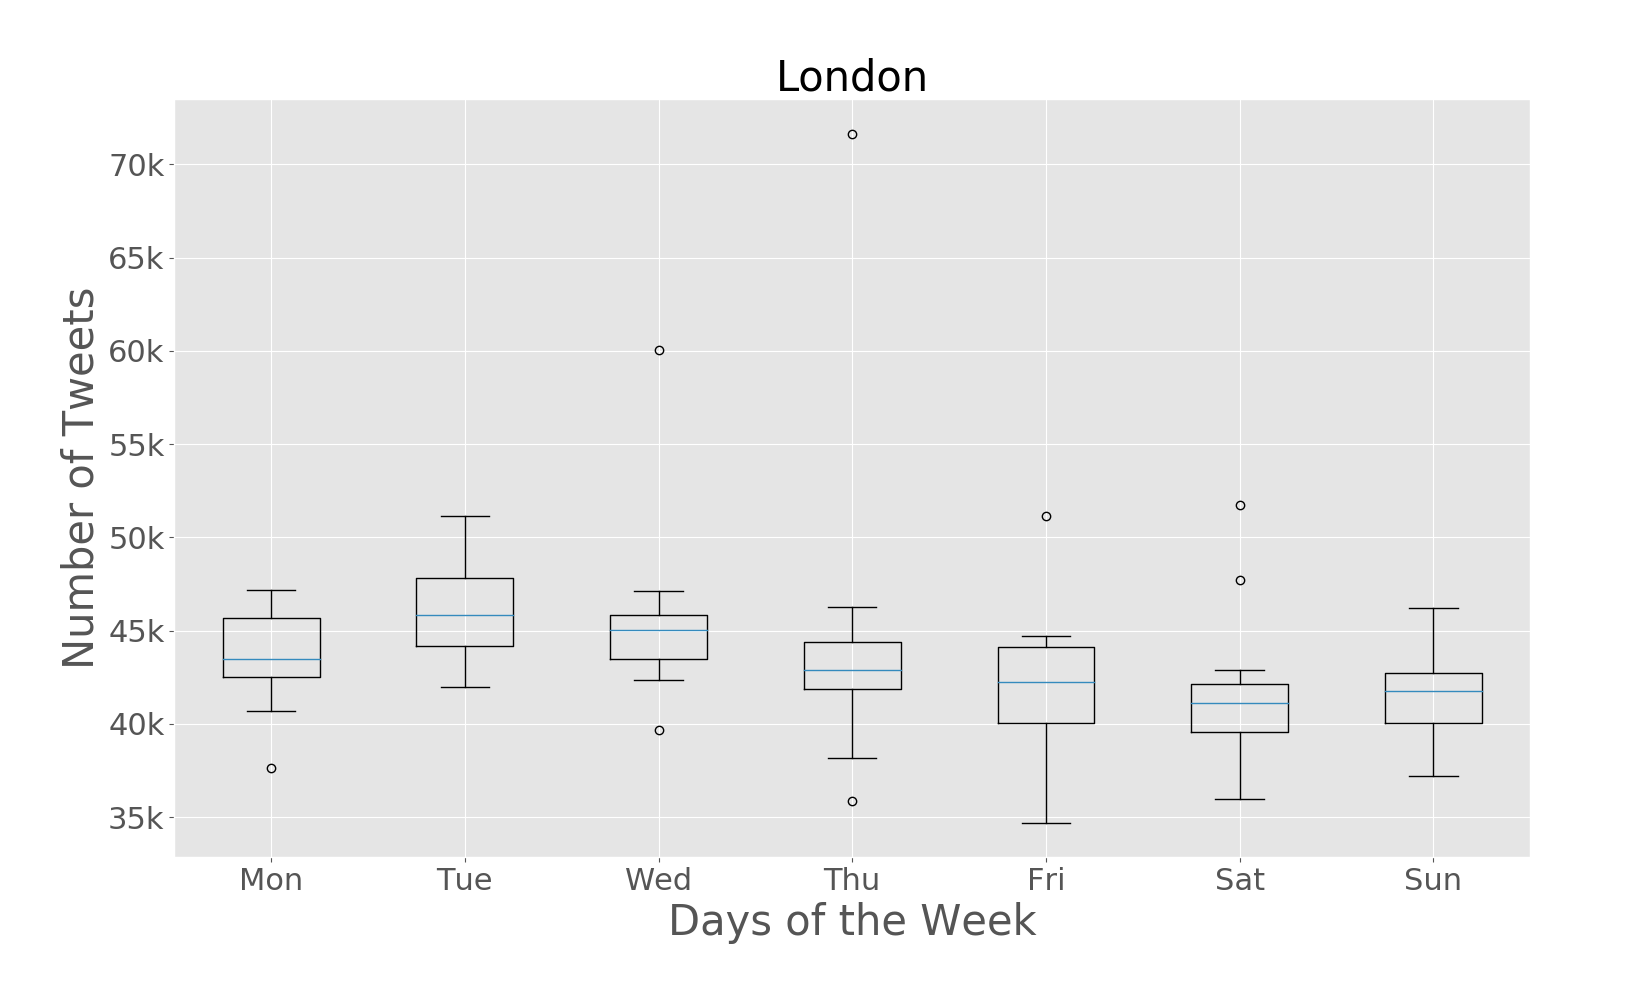
\includegraphics[width=1\linewidth]{figures/london_box_plt_day_of_week.png}
        \caption{}
        \label{subfig:london_box_plot_day_of_week}
    \end{subfigure}

	\medskip
    
     \begin{subfigure}[htbp]{0.45\textwidth}
        \centering
        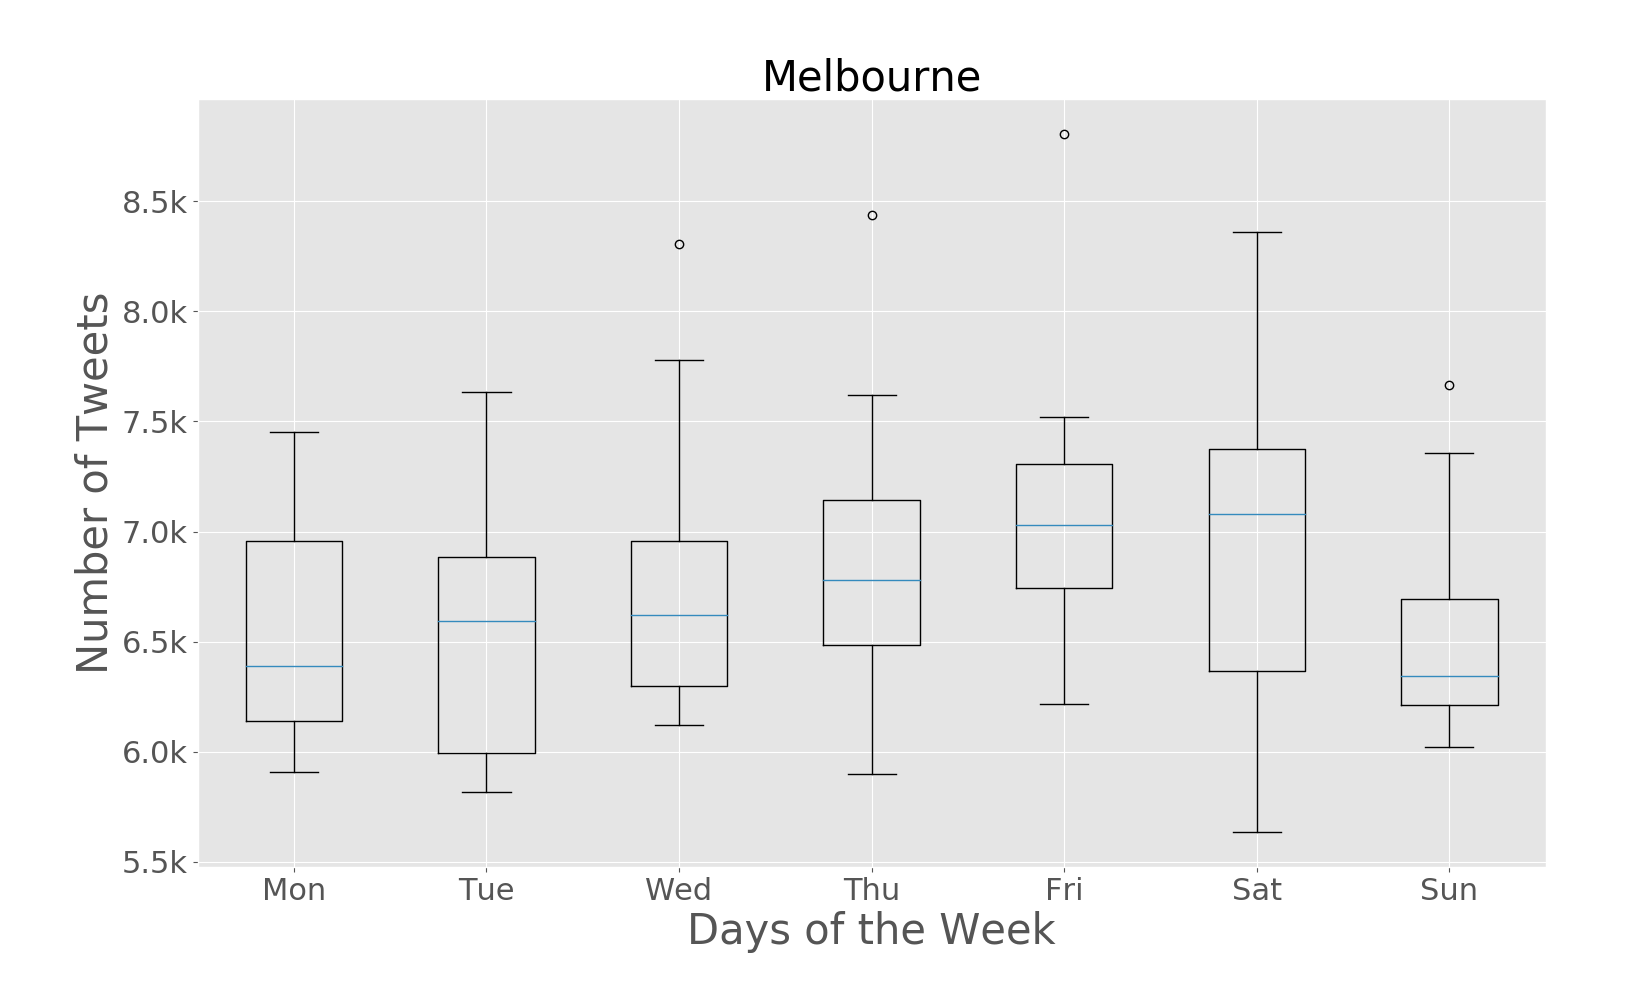
\includegraphics[width=1\linewidth]{figures/melbourne_box_plt_day_of_week.png}
        \caption{}
        \label{subfig:melbourne_box_plot_day_of_week}
    \end{subfigure}
    
\caption[Days-of-the-week box-plots for the volume of tweets]{Days-of-the-week box-plots for the volume of tweets (a) Rio de Janeiro (b) São Paulo (c) New York City (d) London (e) Melbourne}
\label{fig:box_plots_day_of_week}
\end{figure}

In order to understand the most active days and hours in Twitter, for all cities under this study, we aggregate the datasets by these attributes and represented the final results in a box plot representation. This type of data visualization allows, in a standardized way, the displaying of distributions of data based on the six different values: (1) minimum and (2) maximum values for each day/hour regarding the activity on Twitter; (3) median value for the each day/hour, (4) first and (5) third quartiles as well as (6) the interquartile range (IQR). Figures~\ref{fig:box_plots_day_of_week} and~\ref{fig:box_plots_hour_of_day} illustrated this type of data visualization for the whole three months of data collected. Taking into analysis the city of Rio de Janeiro, it was possible to observe and enhance Tuesdays as the day of the week where there is more activity on Twitter. Moreover, Fridays revealed to be the day less active, not only for the city of Rio de Janeiro, but for all remaining cities with exception of Melbourne. Particularly, the activity on Twitter in Melbourne is centered in the weekend days while the other cities the highest levels of activity is spread between week and weekend days. The interquartile range in the plots can tell us the amount of days whose activity was above and behold the median value, and through that we identify Rio de Janeiro and Melbourne as the cities where this phenomenon happen more times. São Paulo, New York City and London present an almost regular IQR which means that the days of weeks are similarly regarding the activity on Twitter.

\begin{figure}[htbp]
	\centering
	\begin{subfigure}[htbp]{0.45\textwidth}
		\centering
		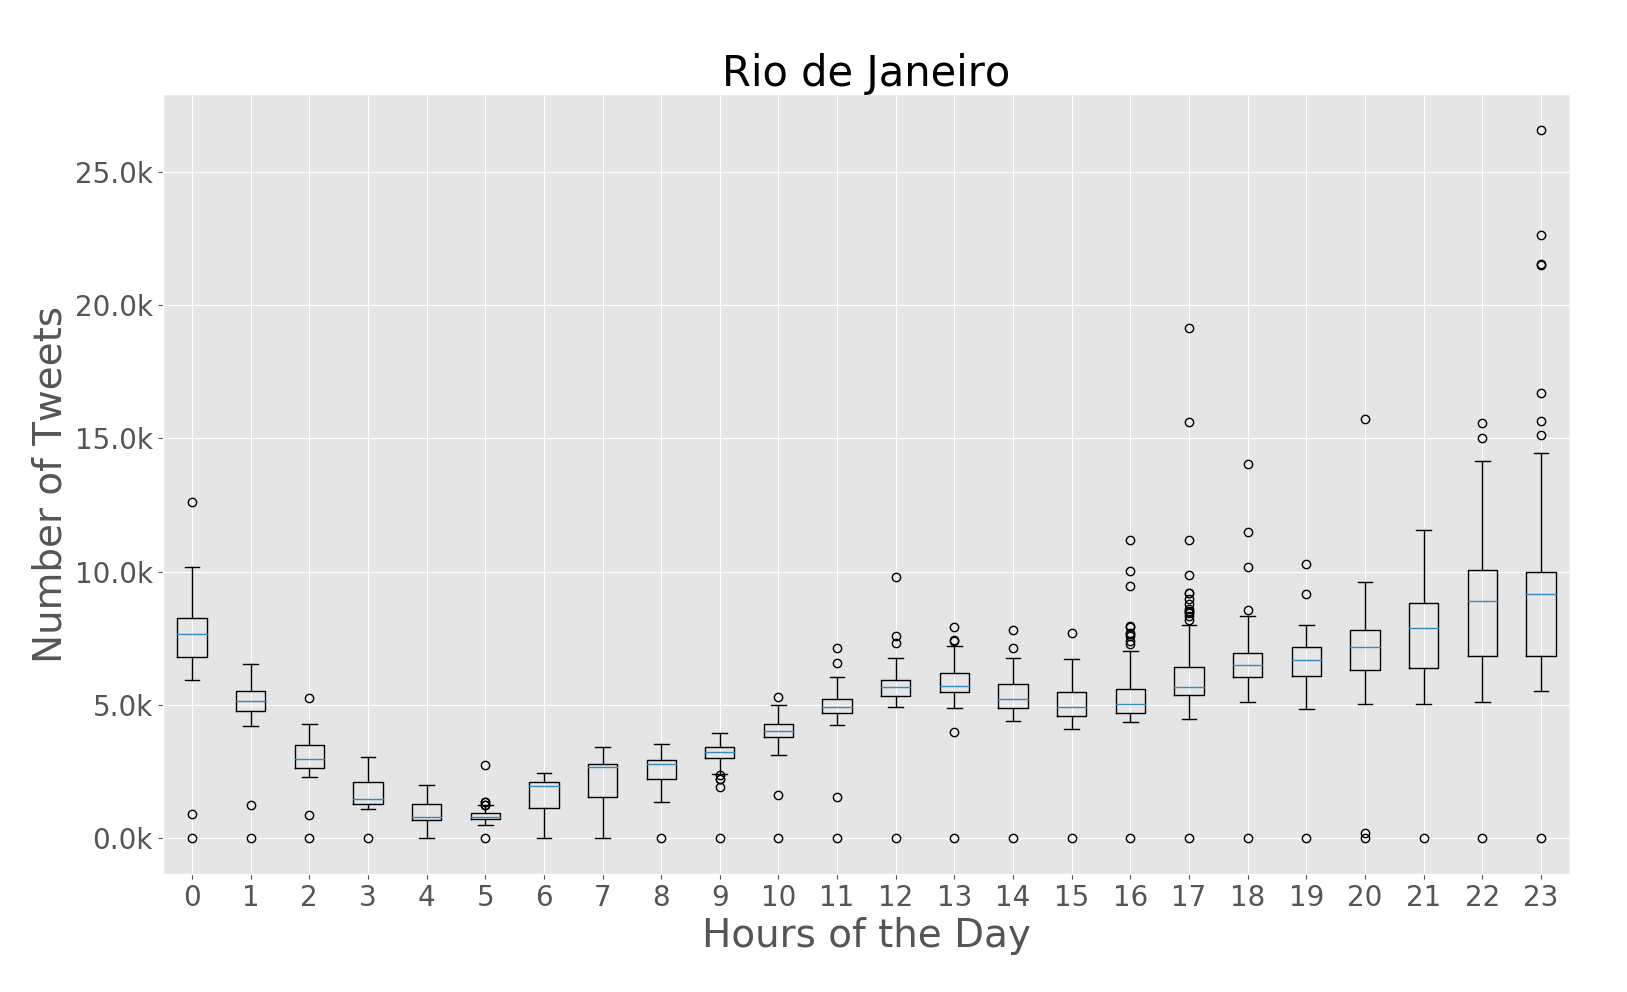
\includegraphics[width=1\linewidth]{figures/rio_box_plt_hour_of_day.png}
		\caption{}
		\label{subfig:riodejaneiro_box_plot_hour_of_day}
	\end{subfigure}%
	\quad
	\begin{subfigure}[htbp]{0.45\textwidth}
		\centering
		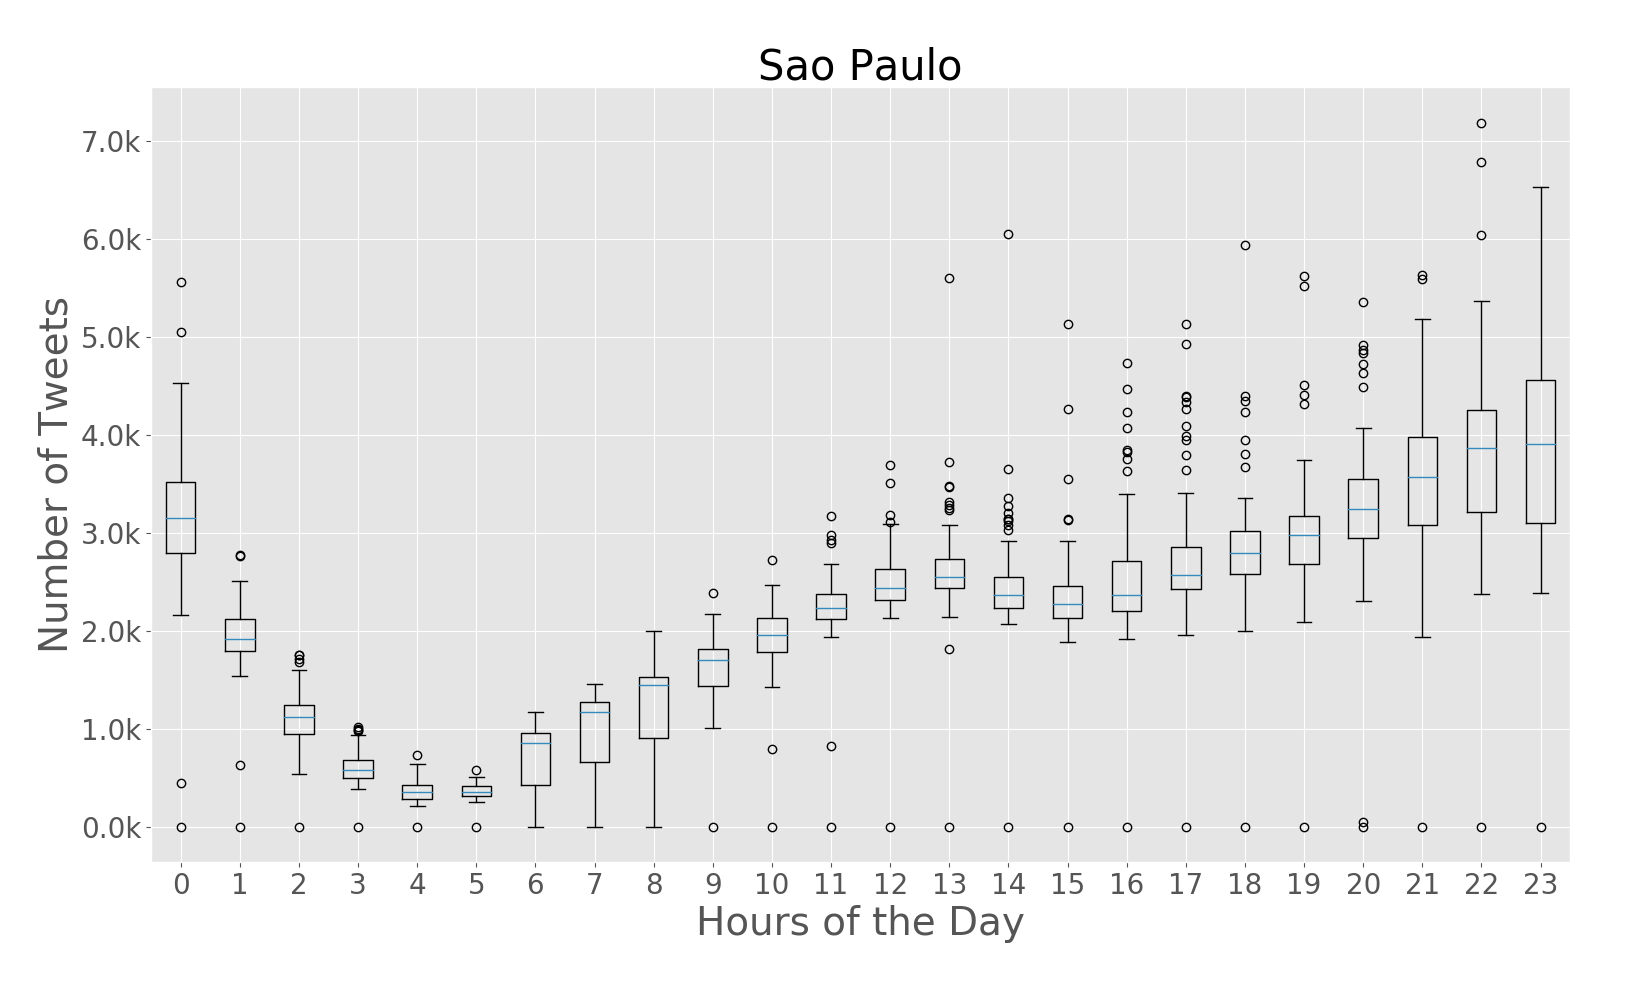
\includegraphics[width=1\linewidth]{figures/sp_box_plt_hour_of_day.png}
		\caption{}
		\label{subfig:saopaulo_box_plot_hour_of_day}
	\end{subfigure}
	
	\medskip
	
	\begin{subfigure}[htbp]{0.45\textwidth}
		\centering
		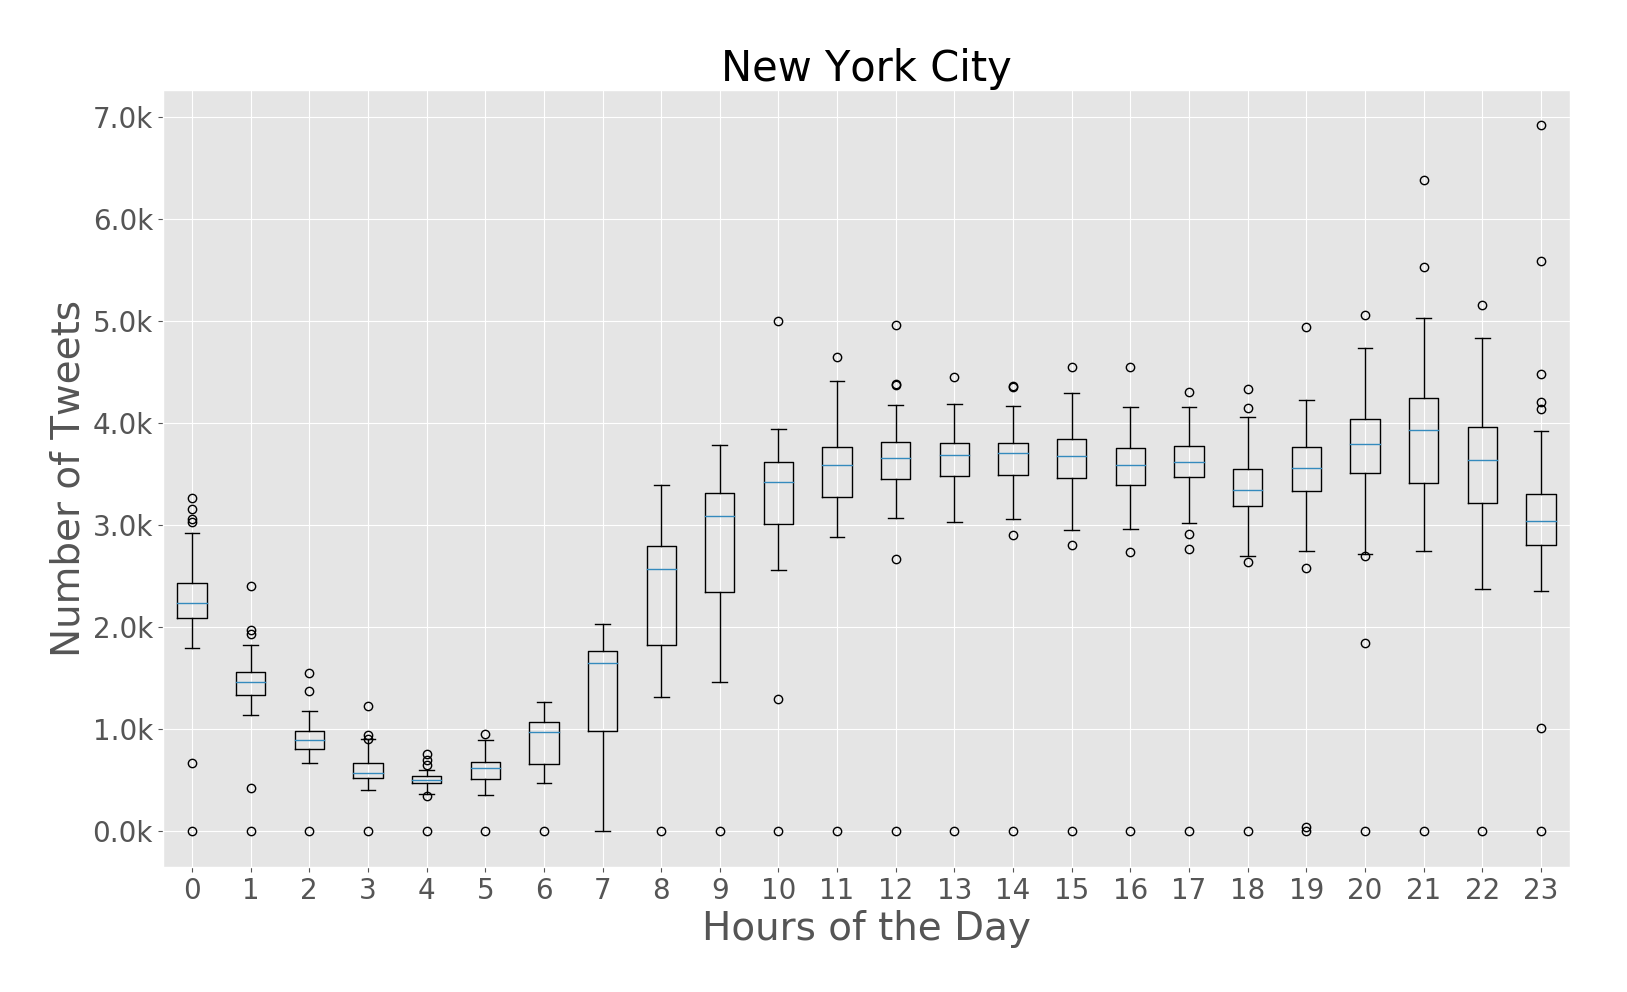
\includegraphics[width=1\linewidth]{figures/nyc_box_plt_hour_of_day.png}
		\caption{}
		\label{subfig:newyork_box_plot_hour_of_day}
	\end{subfigure}
	\quad
	\begin{subfigure}[htbp]{0.45\textwidth}
		\centering
		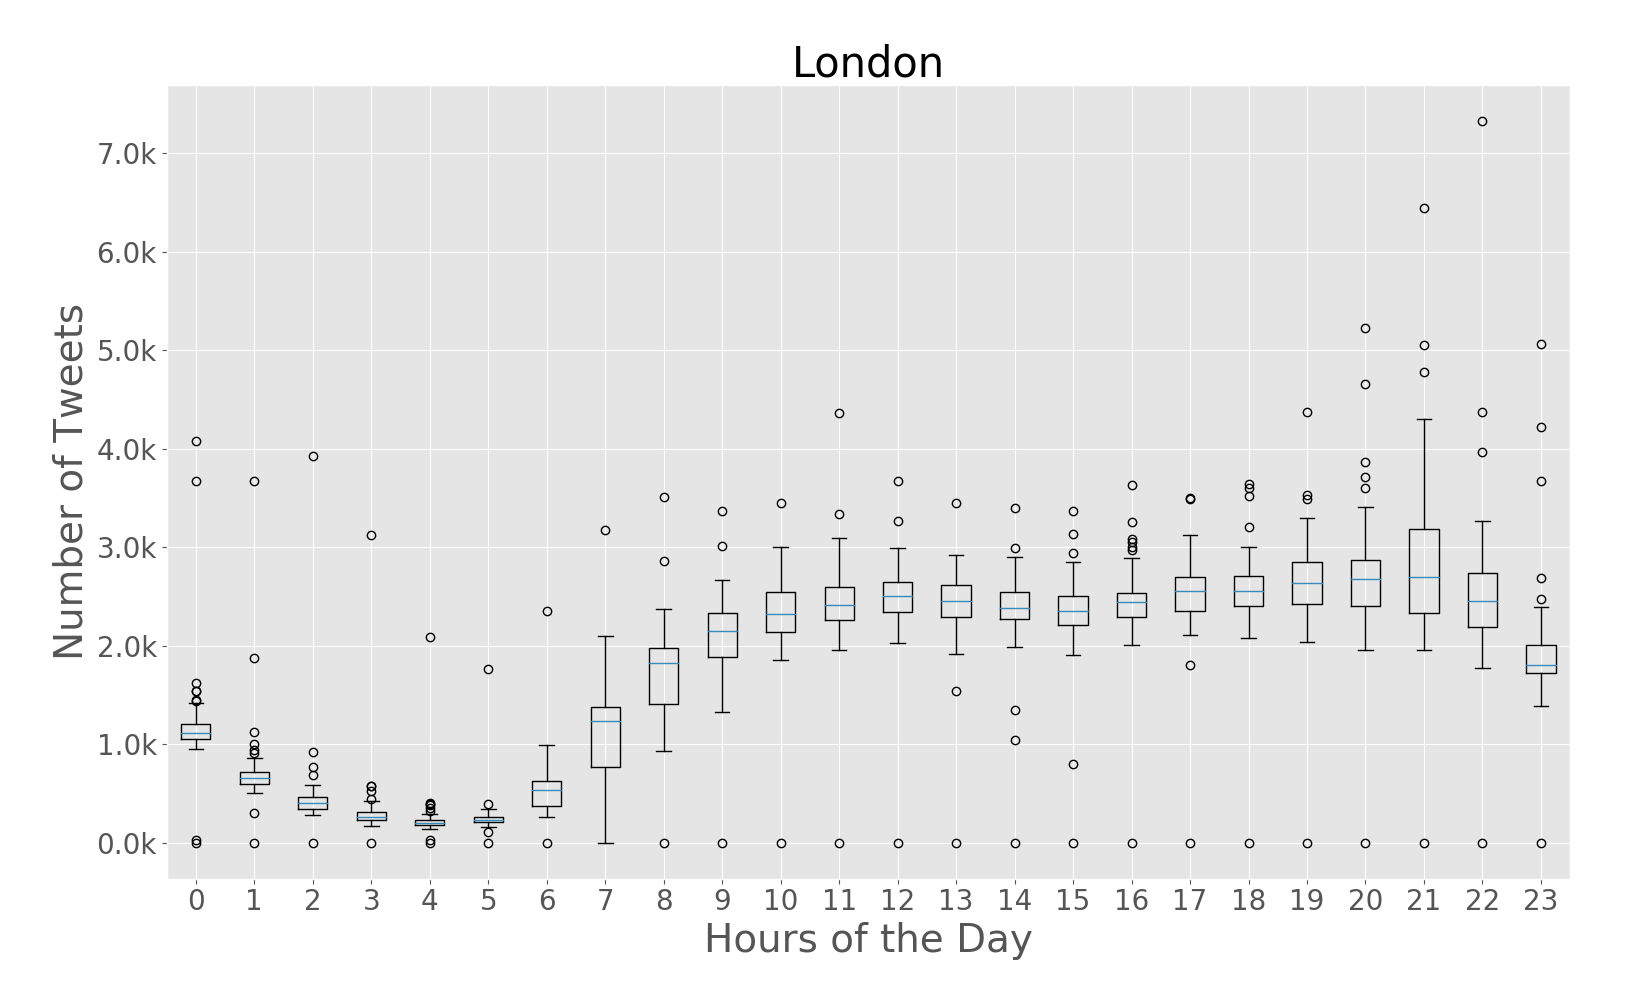
\includegraphics[width=1\linewidth]{figures/london_box_plt_hour_of_day.png}
		\caption{}
		\label{subfig:london_box_plot_hour_of_day}
	\end{subfigure}
	
	\medskip
	
	\begin{subfigure}[htbp]{0.45\textwidth}
		\centering
		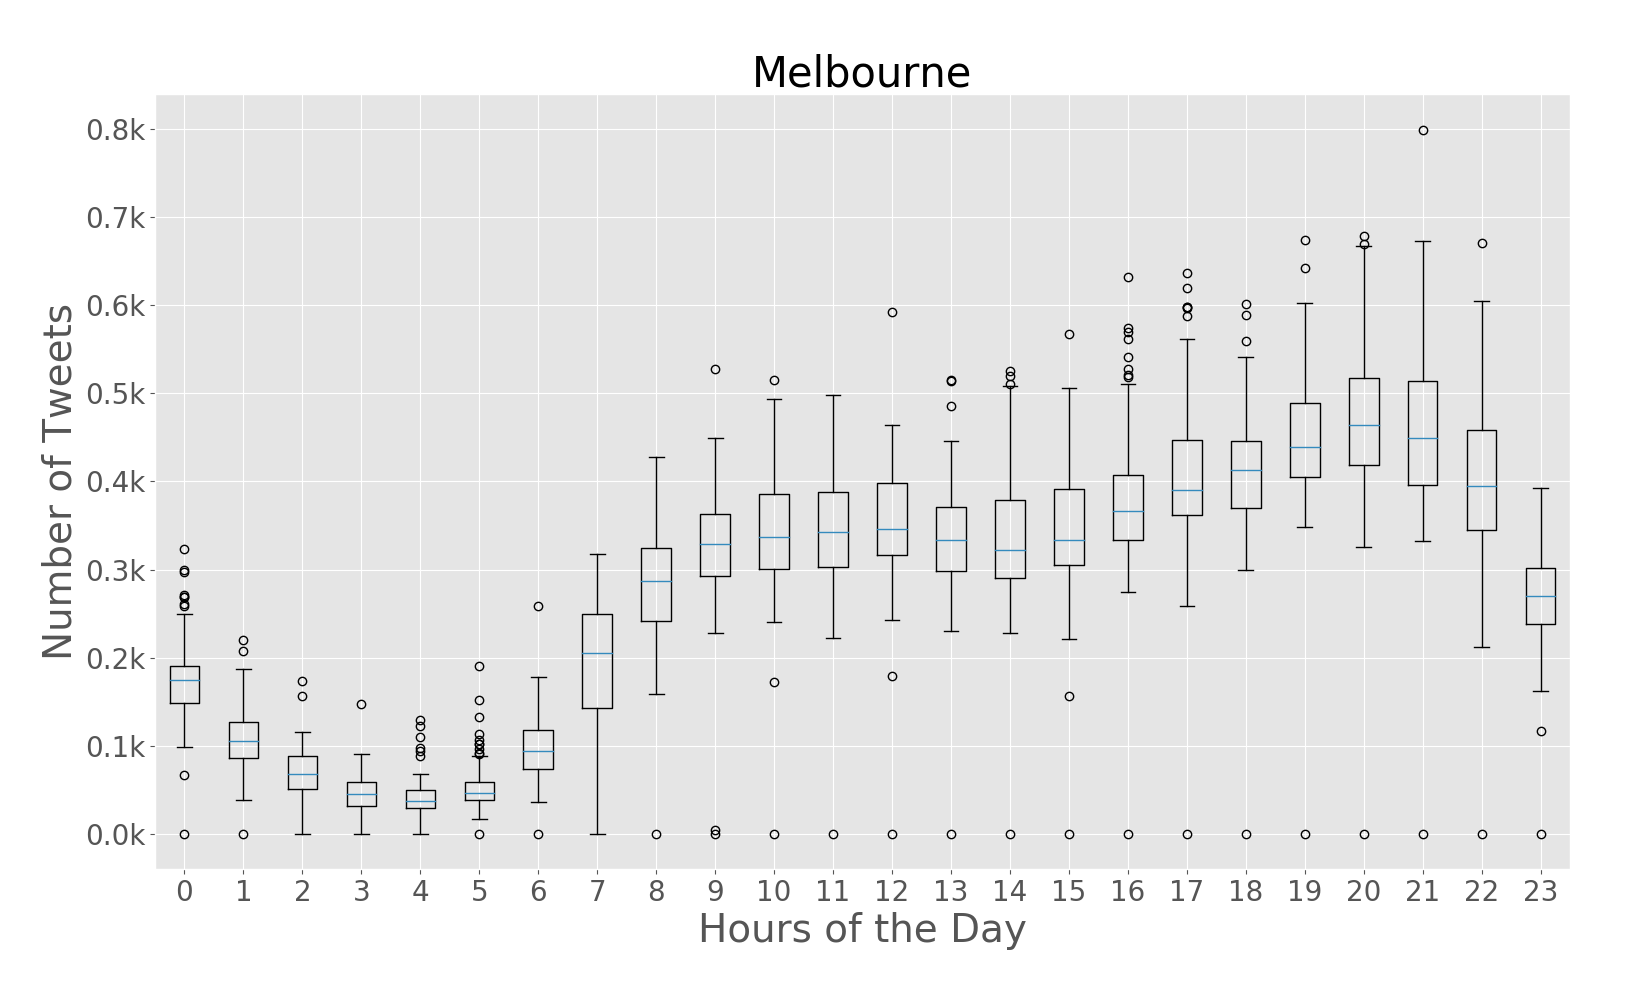
\includegraphics[width=1\linewidth]{figures/melbourne_box_plt_hour_of_day.png}
		\caption{}
		\label{subfig:melbourne_box_plot_hour_of_day}
	\end{subfigure}
	
	\caption[Hour-of-the-day box-plots for the volume of tweets]{Hour-of-the-day box-plots for the volume of tweets (a) Rio de Janeiro (b) São Paulo (c) New York City (d) London (e) Melbourne}
	\label{fig:box_plots_hour_of_day}
\end{figure}

Looking at the hour-of-the-day box-plot (\ref{fig:box_plots_hour_of_day}), it is possible to verify an decrease in terms of activity on Twitter during the night period to all cities. More specifically, there were cases in which the volume of tweets was inexistent and based on this fact, two possible reason are suggested: (1) the absence of tweets during this period is explained through the zero activity of users in the city, regarding geo-located tweets; (2) the service on Twitter was in maintenance and due to that, any tweet was retrieved by the API. Although the observable increase of activity during day-time, the peak of it is similiar to all cities and it is established between the 19 and 23 hours.

\section{Content Composition}

Tweets although its classification as text messages, also contain other kind of \textit{metadata} which exploration of it can sometimes be transformed in added-value information. The \textit{metadata} present in a tweet is represented by the \textit{hashtags}, \textit{user mentions}, \textit{URLs} and \textit{media} attached to it. Other point to explore is the number of distinct users that contributed to the datasets composition. Users which number of posts are unnatural may sometimes be \textit{bots}. If there is a time pattern associated to the post of tweets by a user, for example, the user posts a tweet in a period of 5 minutes over the whole day, then this user is a potential \textit{bot}. The existence of \textit{bots} is not considered in this dissertation because the information provide by such automatic system can also be valuable. In this subsection, we demonstrated the distribution of users over the number of posts made by themselves, as well as the counts of the different type of \textit{metadata }contained in the data. 

Social media platforms present similar characteristics between themselves. One of the most studied ones is the behviour of the its users activity in its services (social media services). The visualization of users activity usually is similar to the power-law distribution long tail~\cite{muchnik2013origins}. Here, we tried to reproduce such visualization in order to establish this kind of correlation as so to prove this behaviour over social media services. The results are present in Figure~\ref{fig:loglog-plots-users}. Each city proved to have a high number of users with few posts and that is observable in the long-tail showed in the cities corresponding sub-figures (~\ref{subfig:riodejaneiro_loglog_users},~\ref{subfig:saopaulo_loglog_users},~\ref{subfig:newyork_loglog_users},~\ref{subfig:london_loglog_users},~\ref{subfig:melbourne_loglog_users}).

The counts and percentages of users that have posted a certain number of tweets was calculated in order to assure the trustiness of the aforementioned distribution. Rio de Janeiro although the highest number of tweets in the datasets only was composed by 135,449 distinct users followed by São Paulo with a lower number 110,352 individuals. The English speaking cities revealed to be very different comparatively to the Portuguese speaking cities in this factor. New York City dataset was composed by 279,554 distinct users, London presented 266,128 users and Melbourne only was composed by 31,733 individuals. Looking at these numbers, we may conclude that Rio de Janeiro has a high percentage of users with more than a certain number of tweets and following this assumption, the log-log distribution made to correlate the behaviour of a power-law distribution must be different from the other cities, at least the English speaking ones.

For example, the percentage of users that posted 20 tweets in a period of three months was almost 63\% for the city of Rio de Janeiro, São Paulo registered 75\%, New York City presented 84\%, London showed 87\% while Melbourne had 87\% of his users with that number of tweets shared. Only taking this example in consideration we proved the assumption mentioned before. The distributions also presented differences if the x-axis is considered. The scale at such axis is one magnitude higher for the English speaking cities, and this means that the number of users with lower number of tweets posted in a three months period is much higher than the users with the same number for the city of Rio de Janeiro.

\begin{figure}[h]
	\centering
	\begin{subfigure}[t]{0.45\textwidth}
		\centering
		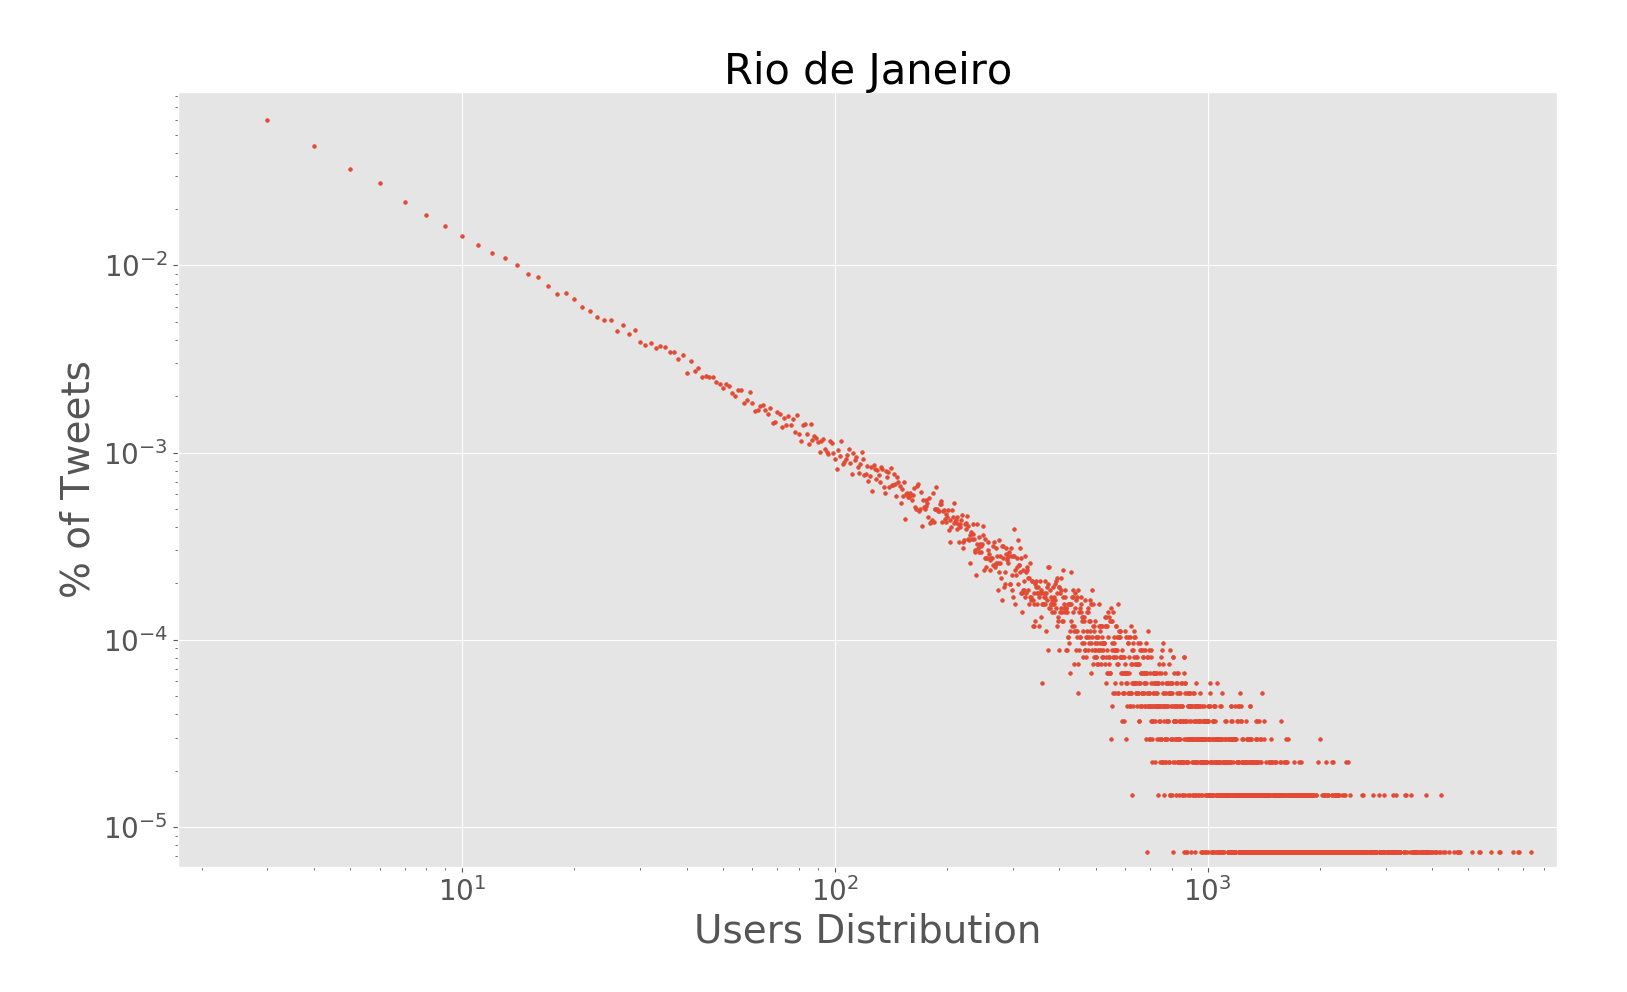
\includegraphics[width=1\linewidth]{figures/rio_loglog_users.png}
		\caption{}
		\label{subfig:riodejaneiro_loglog_users}
	\end{subfigure}%
	\quad
	\begin{subfigure}[t]{0.45\textwidth}
		\centering
		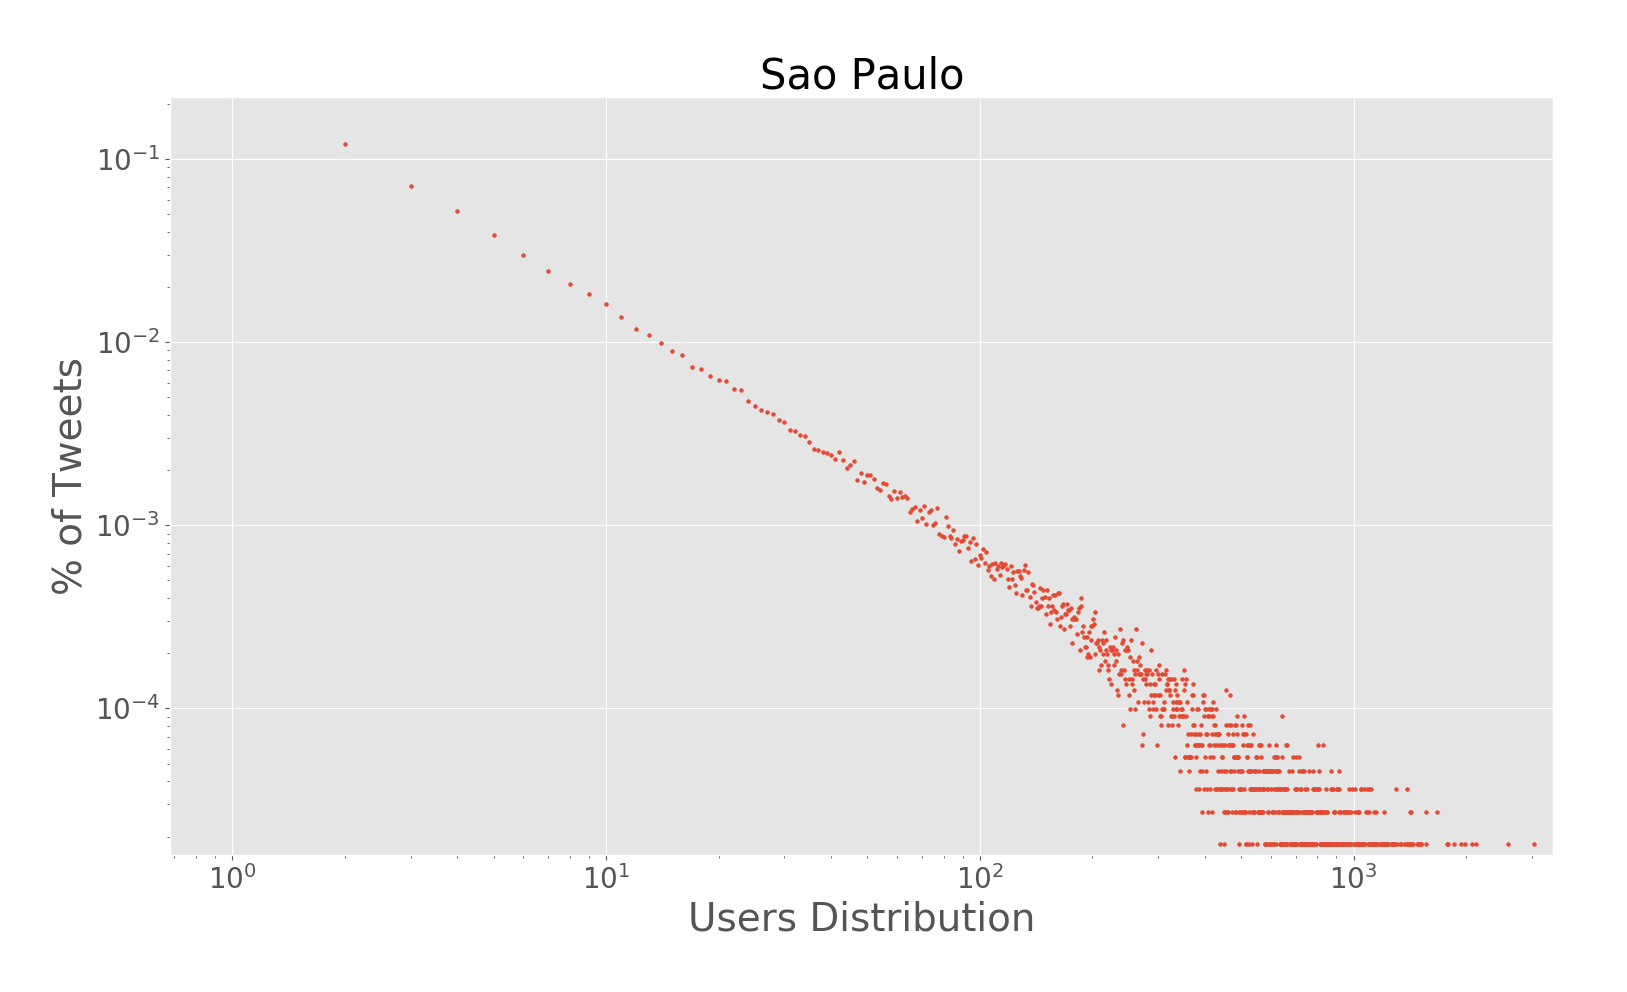
\includegraphics[width=1\linewidth]{figures/sp_loglog_users.png}
		\caption{}
		\label{subfig:saopaulo_loglog_users}
	\end{subfigure}
	
	\medskip
	
	\begin{subfigure}[t]{0.45\textwidth}
		\centering
		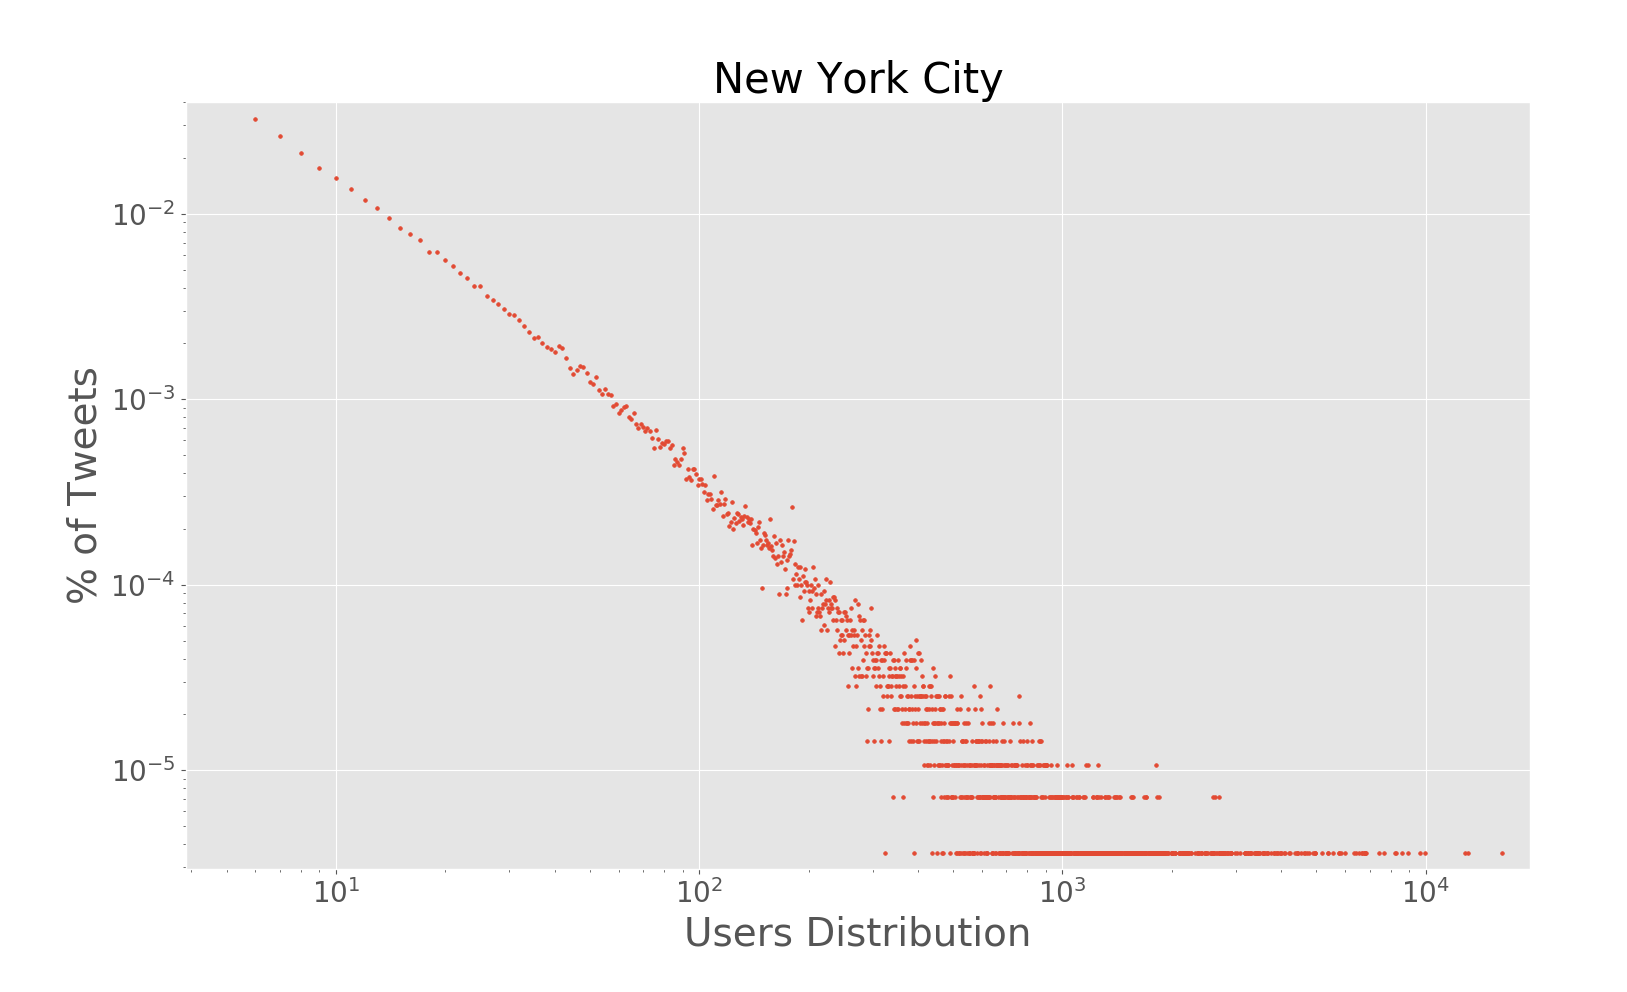
\includegraphics[width=1\linewidth]{figures/nyc_loglog_users.png}
		\caption{}
		\label{subfig:newyork_loglog_users}
	\end{subfigure}
	\quad
	\begin{subfigure}[t]{0.45\textwidth}
		\centering
		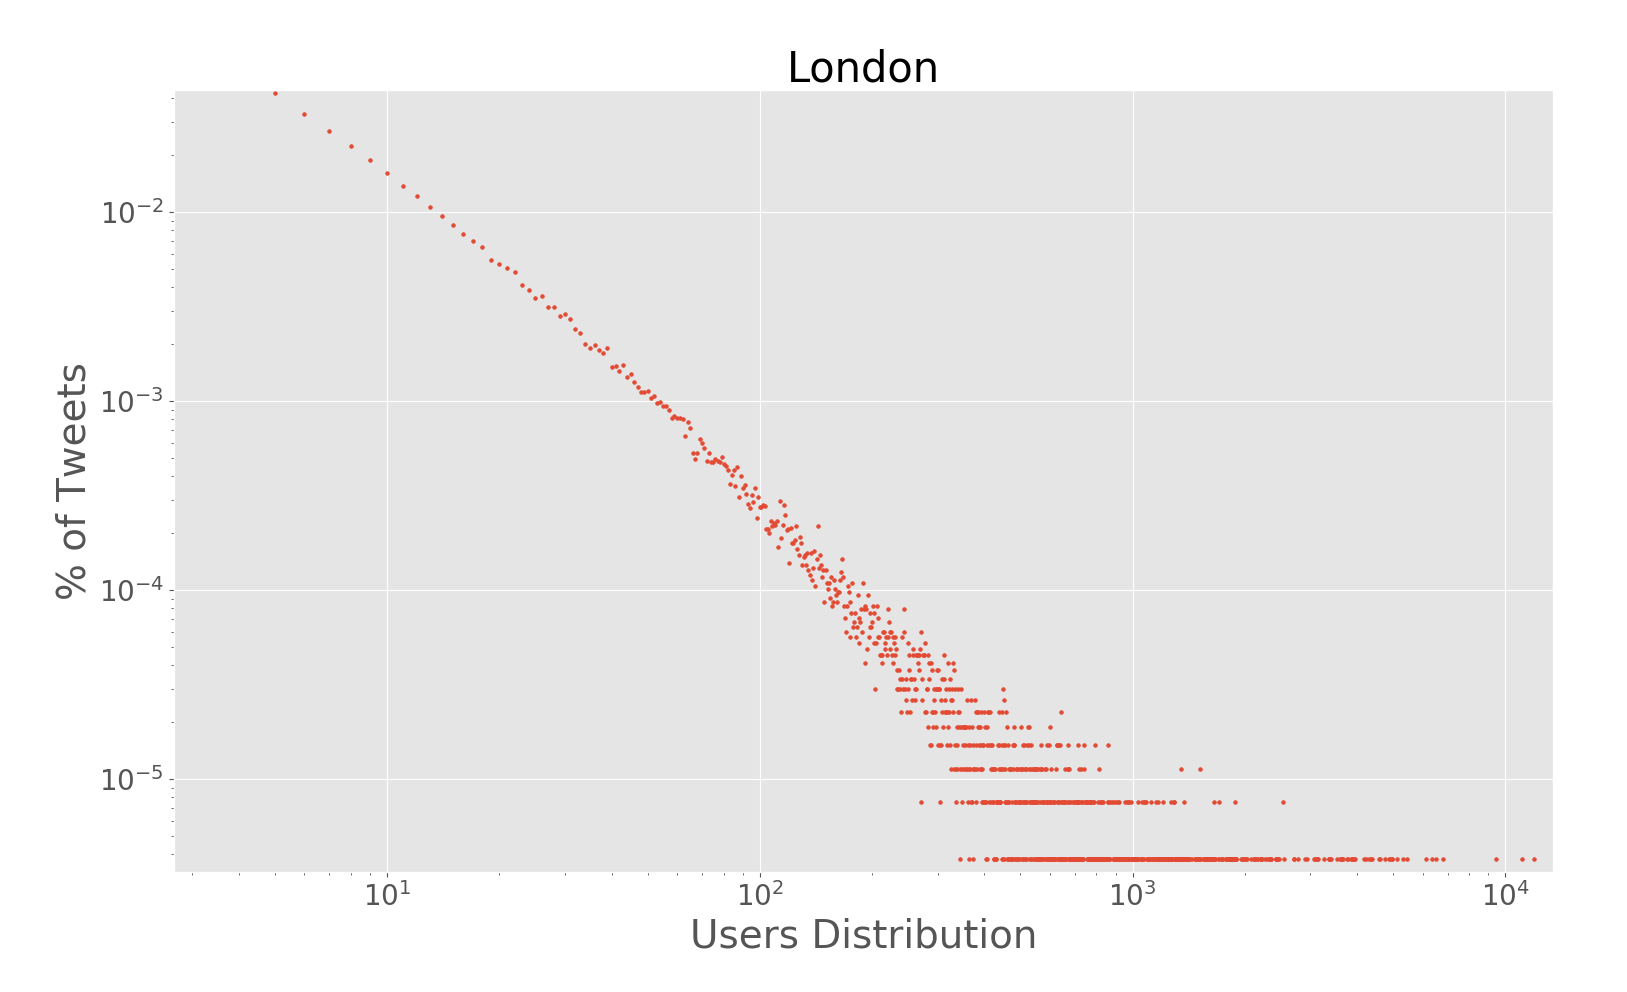
\includegraphics[width=1\linewidth]{figures/london_loglog_users.png}
		\caption{}
		\label{subfig:london_loglog_users}
	\end{subfigure}
	
	\medskip
	
	\begin{subfigure}[t]{0.45\textwidth}
		\centering
		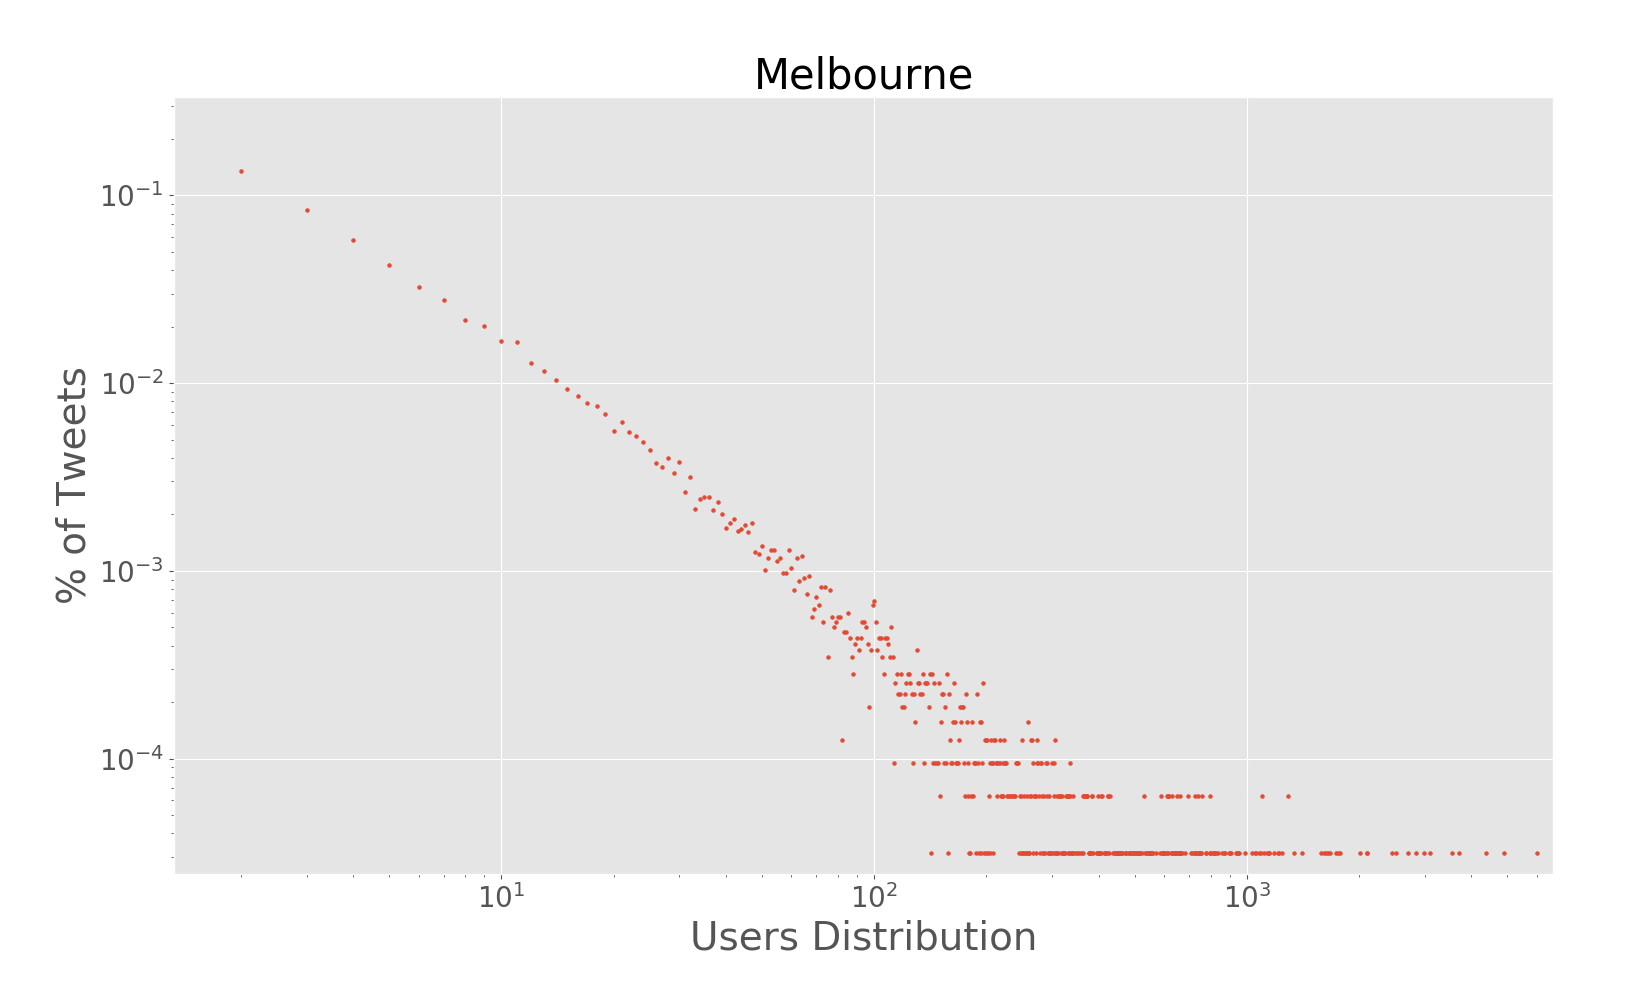
\includegraphics[width=1\linewidth]{figures/melbourne_loglog_users.png}
		\caption{}
		\label{subfig:melbourne_loglog_users}
	\end{subfigure}
	
	\caption[Log-log plots of users distribution]{Log-log plots for the users distribution over the number of tweets posted (a) Rio de Janeiro (b) São Paulo (c) New York City (d) London (e) Melbourne}
	\label{fig:loglog-plots-users}
\end{figure}

The last analysis presented in this subsection is related to the \textit{metadata} contained in the tweets. Here, we want to characterize the different cities with respect to the amount of extra content used by the users in the posts and what kind of information such results suggests for each city.

Having this considered, we counted the volume of each element constituting the previously mentioned \textit{metadata} and calculate the percentage of tweets containing it. In Table~\ref{tab:metadata} are listed the counts and the corresponding percentage of it relatively to the datasets. The resulting analysis and results were performed over the tweets with the city's native language and located inside the bounding-box area used in the filtering process.
The most observable evidence in the results is the greater use of this elements in the English speaking cities. User mentions, as well as \textit{URLs} are the most used \textit{metadata}. This elements may suggest that citizens tend to tag other people in their messages when posting and also share information about certain topic through urls. Regarding the Brazilian cities, the \textit{metadata} usage is not so noticeable. This fact may me related to the number of users composing each dataset because, as it was previously mentioned, the English speaking cities possesses almost two times more users than the Brazilian cities and this characteristic contributes to the increase of this type of \textit{metadata} usage since when someone tag another one in a message, usually a re-post is sent tagging the person responsible by the starting of the conversation. To prove this so, an intensive study about social media tracking and mapping of the flow of each Twitter conversation is needed.

\begin{table}[htbp]
	\centering
	\caption{Percentage of Metadata composing the datasets}
	\label{tab:metadata}
	\resizebox{\textwidth}{!}{\begin{tabular}{l|c|cc|cc|cc|cc}
		\hline
		\multicolumn{1}{c|}{\multirow{2}{*}{\textbf{City}}} & \multicolumn{1}{l|}{\multirow{2}{*}{\textbf{Total}}} & \multicolumn{2}{c|}{\textbf{Hashtags (\#)}} & \multicolumn{2}{c|}{\textbf{User Mentions (@)}} & \multicolumn{2}{c|}{\textbf{URLs}} & \multicolumn{2}{c|}{\textbf{Media}} \\ \cline{3-10} 
		\multicolumn{1}{c|}{} & \multicolumn{1}{l|}{} & \multicolumn{1}{c|}{\textbf{Total (tweets)}} & \textbf{\%} & \multicolumn{1}{c|}{\textbf{Total (tweets)}} & \textbf{\%} & \multicolumn{1}{c|}{\textbf{Total(tweets)}} & \textbf{\%} & \multicolumn{1}{c|}{\textbf{Total (tweets)}} & \textbf{\%} \\ \hline
		\textbf{Rio de Janeiro} & 11,060,136 & 504,835 & 4,56\% & 1,336,329 & 12,08\% & 1,783,060 & 16,12\% & 409,500 & 3,70\% \\
		\textbf{São Paulo} & 4,886,626 & 593,952 & 12,15\% & 1,030,341 & 21,08\% & 1,111,749 & 22,75\% & 325,385 & 6,66\% \\
		\textbf{New York City} & 5,956,355 & 1,697,416 & 28,50\% & 1,752,839 & 29,43\% & 2,839,794 & 47,68\% & 535,945 & 9,00\% \\
		\textbf{London} & 4,040,092 & 1,163,981 & 28,81\% & 1,744,051 & 43,17\% & 1,812,152 & 44,85\% & 465,610 & 11,52\% \\
		\textbf{Melbourne} & 629,424 & 195,967 & 31,13\% & 271,970 & 43,21\% & 258,278 & 41,03\% & 65,941 & 10,48\% \\ \hline
	\end{tabular}}
\end{table}

\section{Summary}
In this chapter we tried to identify interesting patterns and valuable information recurring only to the simple characteristics provided by a tweet: location, date of creation and \textit{metadata} content. First, it was possible to find out existing problems regarding the collection of geo-located tweets. More than one problem is mentioned and possible solutions were designed to surpass them. Our datasets represent only three months of data, however supporting in the analysis made, we conclude that the majority of tweets are tagged with variable sized bounding-boxes instead of precisely geo-coordinates. Furthermore, we tried to instigate temporal patterns using the, already, filtered tweets and proved that it is possible to learnt about remarkable events only seeing abrupt activity on Twitter for some days. By studying the Twitter users distribution it was possible correlate the behaviour of it with the famous power-law distribution. Last but not least, a brief analysis of the \textit{metadata} was performed in order to see the amount of possible topics identified on it (hashtags), the volume of tweets mentioning another user and how many information can be share through the use of urls in this microblog, named Twitter.